\documentclass[aos,preprint]{imsart}

%% Packages
\RequirePackage{amsthm,amsmath,amsfonts,amssymb,multirow,bbm}
%\RequirePackage[numbers]{natbib}
\RequirePackage[authoryear]{natbib} %% uncomment this for author-year bibliography
\RequirePackage[colorlinks,citecolor=blue,urlcolor=blue]{hyperref}
\RequirePackage{graphicx,graphics,epstopdf}
\RequirePackage{soul}
\newcommand{\Yao}[1]{{\textcolor{red}{[Yao: #1]}}}% added by Yao 10/15/2020

\startlocaldefs
%%%%%%%%%%%%%%%%%%%%%%%%%%%%%%%%%%%%%%%%%%%%%%
%%                                          %%
%% Uncomment next line to change            %%
%% the type of equation numbering           %%
%%                                          %%
%%%%%%%%%%%%%%%%%%%%%%%%%%%%%%%%%%%%%%%%%%%%%%
%\numberwithin{equation}{section}
%%%%%%%%%%%%%%%%%%%%%%%%%%%%%%%%%%%%%%%%%%%%%%
%%                                          %%
%% For Axiom, Claim, Corollary, Hypothezis, %%
%% Lemma, Theorem, Proposition              %%
%% use \theoremstyle{plain}                 %%
%%                                          %%
%%%%%%%%%%%%%%%%%%%%%%%%%%%%%%%%%%%%%%%%%%%%%%
%\theoremstyle{plain}
\newtheorem{axiom}{Axiom}
\newtheorem{claim}[axiom]{Claim}
\newtheorem{theorem}{Theorem}[section]
\newtheorem{lemma}[theorem]{Lemma}
\newtheorem{assumption}[theorem]{Assumption}
%%%%%%%%%%%%%%%%%%%%%%%%%%%%%%%%%%%%%%%%%%%%%%
%%                                          %%
%% For Assumption, Definition, Example,     %%
%% Notation, Property, Remark, Fact         %%
%% use \theoremstyle{remark}                %%
%%                                          %%
%%%%%%%%%%%%%%%%%%%%%%%%%%%%%%%%%%%%%%%%%%%%%%
\theoremstyle{remark}
\newtheorem{definition}[theorem]{Definition}
\newtheorem*{remark}{Remark}
\newtheorem*{example}{Example}
\newtheorem*{fact}{Fact}
%%%%%%%%%%%%%%%%%%%%%%%%%%%%%%%%%%%%%%%%%%%%%%
%% Please put your definitions here:        %%
%%%%%%%%%%%%%%%%%%%%%%%%%%%%%%%%%%%%%%%%%%%%%%
\endlocaldefs

\begin{document}

\begin{frontmatter}
\title{supplementary material for "manifold fitting by ridge estimation: a subspace-constrained approach"}
%\title{A sample article title with some additional note\thanksref{t1}}
\runtitle{Manifold fitting by ridge estimation}
%\thankstext{T1}{A sample additional note to the title.}

\begin{aug}
%%%%%%%%%%%%%%%%%%%%%%%%%%%%%%%%%%%%%%%%%%%%%%
%%Only one address is permitted per author. %%
%%Only division, organization and e-mail is %%
%%included in the address.                  %%
%%Additional information can be included in %%
%%the Acknowledgments section if necessary. %%
%%%%%%%%%%%%%%%%%%%%%%%%%%%%%%%%%%%%%%%%%%%%%%
%\author{\fnms{Zhigang} \snm{Yao}\thanksref{t1}\ead[label=e1]{zhigang.yao@nus.edu.sg}},
\author{\fnms{Zhigang} \snm{Yao}\ead[label=e1]{zhigang.yao@nus.edu.sg}},
\and
\author{\fnms{Zheng} \snm{Zhai}\ead[label=e2]{stazhai@nus.edu.sg}}
%\thankstext{t1}{Supported in part by Singapore MOE Tier 1 funding (R-155-000-210-114) and Tier 2 funding (R-155-xxx-xxx-xxx).}
%\thankstext{t2}{Correspondence can be addressed to: zhigang.yao@nus.edu.sg or stazhai@nus.edu.sg}
%\and
%\author[B]{\fnms{Third} \snm{Author}\ead[label=e3]{third@somewhere.com}}
%%%%%%%%%%%%%%%%%%%%%%%%%%%%%%%%%%%%%%%%%%%%%%
%% Addresses                                %%
%%%%%%%%%%%%%%%%%%%%%%%%%%%%%%%%%%%%%%%%%%%%%%
\affiliation{National University of Singapore}
%\address[A,B]{National University of Singapore} 
%\printead{e1,e2}
%}

%\address[B]{Department,
%University or Company Name,
%\printead{e2,e3}}
\end{aug}

%\begin{aug}
%\author{\fnms{First} \snm{Author}\thanksref{t1,t2}\ead[label=e1]{first@somewhere.com}},
%\author{\fnms{Second} \snm{Author}\thanksref{t3}\ead[label=e2]{second@somewhere.com}}
%\and
%\author{\fnms{Third} \snm{Author}\thanksref{t1}
%\ead[label=e3]{third@somewhere.com}
%\ead[label=u1,url]{http://www.foo.com}}
%
%\thankstext{t1}{Some comment}
%\thankstext{t2}{First supporter of the project}
%\thankstext{t3}{Second supporter of the project}
%\runauthor{F. Author et al.}
%
%\affiliation{Some University and Another University}
%
%\address{Address of the First and Second authors\\
%usually few lines long\\
%\printead{e1}\\
%\phantom{E-mail:\ }\printead*{e2}}
%
%\address{Address of the Third author\\
%usually few lines long\\
%usually few lines long\\
%\printead{e3}\\
%\printead{u1}}
%\end{aug}

\begin{abstract}
In this supplement we present the technical proofs for the main work. Equation and theorem references made to the main document do not contain letters.
\end{abstract}


%\begin{keyword}[class=MSC2010]
%\kwd[Primary ]{00X00}
%\kwd{00X00}
%\kwd[; secondary ]{00X00}
%\end{keyword}

%\begin{keyword}
%\kwd{Manifold Fitting}
%\kwd{Ridge estimation}
%\kwd{Kernel density estimation}
%\kwd{Derivatives estimation}
%\end{keyword}
%
\end{frontmatter}

%\begin{quote}
%{\bf Keywords}:    Manifold Fitting, Ridge Estimation, Kernel Density Estimation, Derivatives Estimation, Rank-one Modification
%\end{quote}
%\begin{quote} \small
%{\bf AMS 2000 subject classifications}:   Primary 62G05;
%secondary 62G32.
%\end{quote}

%%%%%%%%%%%%%%%%%%%%%%%%%%%%%%%%%%%%%%%%%%%%%%
%% Please use \tableofcontents for articles %%
%% with 50 pages and more                   %%
%%%%%%%%%%%%%%%%%%%%%%%%%%%%%%%%%%%%%%%%%%%%%%
%\tableofcontents

\begin{appendix}
\section{PROOFS FOR MAIN THEOREMS AND LEMMAS}
In this section, we prove all key theorems and lemmas in the order they appear.
\subsection{Ridge Derivative Lemma}
\begin{lemma}{ 
For any $R_1$, $R_2$, and any point $x_1\in R_1$, the pairwise distance from $x_1$ to $R_2$ yields the order of: %$\min_{x_2\in R_2}\|x_1-x_2\|_2$ %between any two ridges $R_1$ and $R_2$ 
%is of order $O(\|H_1(x_1)-H_2(x_1)\|_F+\|g_1(x_1)-g_2(x_1)\|_2)$, 
\[
\min_{x_2\in R_2}\|x_1-x_2\|_2 = O(\|H_1(x_1)-H_2(x_1)\|_F+\|g_1(x_1)-g_2(x_1)\|_2)
\]
where $H_1(x_1), g_1 (x_1)$ are the Hessian and gradient of some estimated density function $p_1(x_1)$ evaluated at $x_1$; $H_2(x_1)$ and $g_2(x_1)$ are the Hessian and gradient of the density function of $p_2(x)$ evaluated at $x_1$, respectively.
%For any two ridges $R, \hat{R}$ defined by $R = \{x| \Pi_{H}(x)g(x) = 0\}$,$\hat{R} = \{x| \Pi_{\hat{H}}(x))\hat{g}(x) = 0\}$, 
 %$d(x, \hat{R}) = O(\|\hat{H}(x)-H(x)\|_F+\|\hat{g}(x)-g(x)\|_2)$
 }\label{margin}
\end{lemma}

The following proof is a revised simple version of a similar proof in \cite{genovese2014nonparametric}. For completeness, we also include it in our paper.

\begin{proof}\label{Ridge Derivative Lemma}
 For two ridges $R_1, R_2$, we have two density functions $p_1(x)$ and $p_2(x)$ such that the points on each ridge satisfy the solution of
 $\Pi_{H_1}(x) g_1(x) = 0$ 
 and $\Pi_{H_2}(x) g_2(x) = 0$ respectively. For any starting point $x_a \in R_1$, we can build a unit speed curve $\gamma(s)$ derived from the gradient and Hessian of $p_2(x)$ as
 \begin{gather*}
 \gamma_2(0) = x_a \in R_1,\\
 \gamma_2(t_0) = x_b \in R_2,\\
 \gamma'_2(s) = \frac{\Pi_{H_2}(\gamma(s))g_2(\gamma(s))}{\|\Pi_{H_2}(\gamma(s))g_2(\gamma(s))\|_2}.
 \end{gather*}
Note that the curve $\gamma(t)$ connect $x_a$ with $R_2$ by $x_b$. Define the univariate function $\xi(s)$ as
  \[
  \xi_2(s) = p_2(\gamma_2(t_0))-p_2(\gamma_2(s)), \quad 0<s<t_0.
  \]
Through a simple computation, we know 
 \[
 \xi'_2(s)=-\langle  g_2(\gamma_2(s)), \gamma'_2(s) \rangle =- \|\Pi_{H_2}(\gamma_2(s))g_2(\gamma_2(s))\|_2, \quad \xi'_2(t_0) = 0.
 \]
 %\[
 %\xi''(s) = \frac{\langle L_{\gamma'(s)}(\gamma(s)) g(\gamma(s)), L(\gamma(s)g(\gamma(s)))\rangle}{\|L(\gamma(s))g(\gamma(s))\|_2}
 %\]
 %with $\gamma(s)=\frac{L(\gamma(s)g(\gamma(s)))}{\|L(\gamma(s)g(\gamma(s)))\|}$
 The distance from $x_a$ to $R_2$ can be bounded by the curve length of $\gamma_2(t)$ which is $t_0$
 \[
 \begin{aligned}
 &d(x_a, R_2) \\
 =& \|x_a-P_{R_2}(x_a)\|_2\\
 \leq& \|x_a-x_b\|_2 \\
 = &\|\gamma_2(t_0)-\gamma_2(0)\|_2\leq t_0.
 \end{aligned}
 \]
Finally, the problem becomes to bound $t_0$. Suppose $\sup_u \xi''_2(u)>\frac{1}{c}$, by the mean-value theorem, we have
 \[
 \begin{aligned}
 t_0 = &\frac{\xi'_2(t_0)-\xi'_2(0)}{\xi''_2(u)} \\
 = &\frac{\|\Pi_{H_2}(\gamma_2(0))g_2(\gamma_2(0))\|_2}{\xi''_2(u)} \\
 \leq & c \|\Pi_{H_2}(\gamma_2(0))g_2(\gamma_2(0))\|_2.
 \end{aligned}
 \]
 Next, we show that $\|\Pi_{H_2}(\gamma_2(0))g_2(\gamma_2(0))\|_2$ is of the same order with an approximation error of $H_2(x)$ and $g_2(x)$:
 \begin{equation}
 \begin{aligned}\label{bound_temp1}
 &\|\Pi_{H_2}(\gamma_2(0))g_2(\gamma_2(0))\|_2\\
 =&  \|\Pi_{H_2}(\gamma_2(0))g_2(\gamma_2(0)) - \Pi_{H_1}(\gamma_2(0))g_1(\gamma_2(0))\|_2
 \end{aligned}
 \end{equation}
 Using the triangle-inequality with respect to the $\|\|_2$ norm, we have \eqref{bound_temp1} is dominated by
 \begin{equation}\label{bound_temp2}
 \begin{aligned}
& \|\Pi_{H_2}(\gamma_2(0))g_2(\gamma_2(0)) -\Pi_{H_1}(\gamma_2(0)){g_2}(\gamma_2(0)) \|_2 +...\\
 & \quad \quad  \quad \quad  \quad \quad + \|\Pi_{H_1}(\gamma_2(0)){g_2}(\gamma_2(0)) - \Pi_{H_1}(\gamma_2(0))g_1(\gamma_2(0))\|_2\\
 \end{aligned}
 \end{equation}
 For any matrix $A$, using the Cauchy-Schwartz inequality on each row of $A$, we will get the result $\|Ax\|_2\leq \|A\|_F\|x\|_2$. Thus, similarly, we have \eqref{bound_temp2} is dominated by
 \[
 \begin{aligned}
 & \|\Pi_{H_2}(\gamma_2(0)) - \Pi_{H_1}(\gamma_2(0))\|_F\|g_2(\gamma_2(0))\|_2 +...\\
 &\quad \quad  \quad \quad  \quad \quad  +\|\Pi_{H_1}(\gamma_2(0))\|_F\|g_2(\gamma_2(0))-g_1(\gamma_2(0))\|_2, \\
 \end{aligned}.
 \]
According to the Davis-Kahan theorem, $\|\Pi_{H_2}(\gamma_2(t))-\Pi_{H_1}(\gamma_2(t))\|_F \leq \beta\|H_2(\gamma_2(t))-H_1(\gamma_2(t))\|_F$. The conclusion is proved!
\end{proof}


\subsection{Derivatives' Bias Bound}\label{bias_proof}
\begin{theorem}
The bias of the first order and second order of the $\hat{p}_h(x)$ is 
\begin{equation*}\label{BiasResult}
|{\rm E}(\partial_{x_s}  \hat{p}_h(x)) - \partial_{x_s}p(x)|  = \frac{h^2|\Delta (\partial_{x_s}p(x))|}{2D}  \int \|u\|_2^2 K(u) du+o(h^2),
\end{equation*}
\begin{equation*}\label{order2}
|{\rm E}( \partial_{x_s} \partial_{x_t}  \hat{p}_h(x)) -  \partial_{x_s} \partial_{x_t} p(x)| = \frac{h^2 |\Delta (\partial_{x_s}\partial_{x_t} p(x))|}{2D} \int \|u\|_2^2 K(u) du+o(h^2).
\end{equation*}
where $\Delta$ is the Laplace-Beltrami operator.
\end{theorem}

\begin{proof}
Suppose the kernel function vanishes at infinity for each dimension, i.e., it satisfies $\lim_{u_s\rightarrow \infty}K(u)=0$ for each dimension. Then, using the integration-by-parts formula, we obtain the expectation of first-order derivatives:
\begin{equation}\label{Expectation}
\begin{aligned}
&{\rm E} (\partial_{x_s} \hat{p}_h(x)) \\
\overset{s.1}{=}& \frac{1}{h^D} \int_{y\in \mathbb{R}^D}{\partial_{x_s}}  K(\frac{x-y}{h}) p(y) dy  \\
\overset{s.2}{=}&\frac{1}{h^{D+1}}\int \partial_{z_s} K(z)|_{z=\frac{x-y}{h}} p(y) dy\\
\overset{s.3}{=}&h^{-1} \int_ {u\in \mathbb{R}^D} \partial_{u_s} K(u) p(x-hu)  d u\\
\overset{s.4}{=}&h^{-1}\int_ {u\in \mathbb{R}^D} K(u) \partial_{u_s} p(x-hu) d u \\
\overset{s.5}{=}& \int_ {u\in \mathbb{R}^D} K(u) \partial_{z_s}p(z)|_{z=x-hu} d u.
\end{aligned}
\end{equation}
%We explain the reason for each steps as: 
The equation $s.1$ is the definition of expectation. The equation $s.2$ is obtained from the derivative of the function composition. The equation $s.3$ is obtained from the formula of integration by changing variables. The equation $s.4$ is obtained from the formula of the integration by partition. The equation $s.5$ is similar with that of equation $s.2$.

For the multivariate function $\partial_{x_s} p(x)$, we have the Taylor expansion of $\partial_{x_s} p(x)$ up to order 2 as
\begin{equation}\label{Taylor}
\begin{aligned}
&\partial_{z_s} p(z)|_{z=x-hu}\\
= &\partial_{x_s} p(x) -  h u^T\nabla \partial_{x_s} p(x) + \frac{1}{2}h^2 u^T H(\partial_{x_s}p(x))u + o(h^2).
\end{aligned}
\end{equation}

Since $u^T \nabla \partial_{x_s} p(x) K(u)$ is an odd function with respect to each variable $u_s$, we have the integration $\int u^T \nabla \partial_{x_s} p(x) K(u) du = 0 $ in a symmetric region. 

For the term $u^T H(\partial_{x_s}p(x))u$, we know it is related with the Laplace Beltrami operator of $\Delta(\partial_{x_s}p(x))$ by
\[
\begin{aligned}
\int u^T H(\partial_{x_s}p(x))u K(u) du =& \langle \int uu^TK(u) du, H(\partial_{x_s}p(x))\rangle\\
\overset{s.6}{=}&\frac{\int \|u\|_2^2K(u)du}{D} \langle  I, H(\partial_{x_s}p(x))\rangle\\
=&\frac{\int \|u\|_2^2K(u)du}{D} \Delta(\partial_{x_s}p(x)),
\end{aligned}
\]
where the equation of $s.6$ is obtained from $\|u\|_2^2 = \sum_k u^2_k$, and
\[
\int u_k u_s K(u)du=0 \quad k\neq s,
\] because of symmetric domain of integration and the independence  for each of the dimensions. 

Combining the above results, we know the bias
\begin{equation}\label{BiasResult}
|{\rm E}(\partial_{x_s} \hat{p}_h(x)) - \partial_{x_s}p(x)|  = \frac{|\Delta(\partial_{x_s} p(x))|}{2D} h^2 \int \|u\|_2^2 K(u) du+o(h^2),
\end{equation}
where $\Delta(\partial_{x_s} p(x))$ is the Laplace-Beltrami operator of $\partial_{x_s} p(x)$, which is also the summation of the diagonal elements of the Hessian matrix $H(\partial_{x_s}p(x))$. Similarly, repeating the same procedure as \eqref{Expectation}\eqref{Taylor}, we have the second-order bias as
%where $\lambda_s(x)$ is the largest eigenvalue of the Hessian matrix $H(\partial_{x_s}p(x))$. 
\begin{equation}\label{order2}
|{\rm E}( \partial_{x_s} \partial_{x_t}   \hat{p}_h(x)) -  \partial_{x_s} \partial_{x_t} p(x)| = \frac{|\Delta(\partial_{x_s}\partial_{x_t} p(x))|}{2D} h^2 \int \|u\|_2^2 K(u) du+o(h^2).
\end{equation}
The same with \eqref{BiasResult}, $\Delta(\partial_{x_s}\partial_{x_t} p(x))$ is the Laplace-Beltrami operator of $\partial_{x_s}\partial_{x_t} p(x)$ which is also the summation of the eigenvalues of the matrix $M_{s,t}$ whose $i,j$-th element is $\frac{\partial^4}{\partial x_s\partial x_t \partial x_i \partial x_j} p(x)$.%, i.e., $\lambda_{st}(x)= \max_k \lambda_k( M_{st}(x))$.
\end{proof}
\subsection{Derivatives' Variance Bound}\label{variance_proof}
\begin{theorem}
The variance of the first and second order derivatives for $\hat{p}_h(x)$ has a bound as 
\begin{equation*}\label{VarResult}
\begin{aligned}
&{\rm E} |\partial_{x_s} \hat{p}_h(x)-{\rm E}(\partial_{x_s} \hat{p}_h(x))| = \sqrt{\frac{\phi_s(x)}{n h^{D+2}}}+O(\frac{1}{n^{1/2}h^{(D+1)/2}}),\\
&{\rm E} | \partial_{x_s}\partial_{x_t} \hat{p}_h(x) -{\rm E}(\partial_{x_s}\partial_{x_t} \hat{p}_h(x))| = \sqrt{\frac{\phi_{s,t}(x)}{nh^{D+4}}}+O(\frac{1}{n^{1/2}h^{(D+3)/2}}).
\end{aligned}
\end{equation*}
%where $M(u) = \partial_{u_s}K(u)$ and $N(u) = \partial_{u_t}\partial_{u_s}K(u)$, respectively.
\end{theorem}

\begin{proof}
Because of the i.i.d. assumption and the characters of the variance, the first-order derivative yields
\[
\begin{aligned}
 &{\rm Var} (\partial_{x_s} \hat{p}_h(x))  \\
 \overset{s.7}{=} &{\rm Var} (\frac{1}{n h^D}\sum_k \partial_{x_s}(K(\frac{x-y_k}{h})))\\
 \overset{s.8} = &\frac{1}{n h^{2D}} {\rm Var}(  \partial_{x_s} K(\frac{x-y}{h}))))\\
 \overset{s.9} = & \frac{1}{n h^{2D+2}} {\rm Var} (\partial_ {u_s}  K(u)|_{u=\frac{x-y}{h}}).%= \frac{1}{n h^{2d+4}} (E_y({k^{''}}^2_{rs}(\frac{x-y}{h}))- E_y^2(k^{''}_{rs}(\frac{x-y}{h}))
\end{aligned}
\]
Similarly as the process derived in the bias, equation $s.7$ is the definition of variance, equation $s.8$ is obtained from the independence of the samples of $y_k$ and equation $s.9$ is because of derivative for the composite functions.

Next, we derive the variance by using the equality of variance and expectation ${\rm Var}(a) = {\rm E}(a^2)-{\rm E}^2(a)$.
In addition, denote $M(\frac{x-y}{h}) = \partial_ {u_s}  K(u)|_{u=\frac{x-y}{h}}$, the variance will lead to
\begin{equation}\label{e11}
\begin{aligned}
 &{\rm Var} (\partial_{x_s} \hat{p}_h(x))\\
  = &\frac{1}{nh^{2D+2}}({\rm E}_y (M^2(\frac{x-y}{h}))-{\rm E}^2_y(M(\frac{x-y}{h}))).
%\frac{1}{h^d}\int M(\frac{x-y}{h}) p(y)dy = \int M(u)p(x-uh) du=p(x) \int M(u) du+O(h)
\end{aligned}
\end{equation}
Noting the bias result from \eqref{Expectation} and \eqref{BiasResult}, we have
\begin{equation}\label{EM}
\begin{aligned}
&{\rm E}_y(M(\frac{x-y}{h})) \\
= &h^{D+1} ( {\rm E}(\partial_{x_s} \hat{p}_h(x))\\
\leq &h^{D+1} (\partial_{x_s} p(x)+\frac{\Delta(\partial_{x_s}p(x))}{2D} h^2 \int \|u\|^2 K(u) du+o(h^2)).
\end{aligned}
\end{equation}
Taking the square of \eqref{EM} on both sides, we obtain
\[
{\rm E}^2_y(M(\frac{x-y}{h})) = h^{2D+2}((\partial_{x_s} p(x))^2+ O(h^2)).
\]
Taking the expectation of $M^2(\frac{x-y}{h})$, and changing the variable $u=\frac{x-y}{h}$, we obtain
\begin{equation}\label{part1}
\begin{aligned}
&{\rm E}_y(M^2(\frac{x-y}{h})) \\
=& \frac{1}{h^D} \int M^2(u) p(x-uh) du \\
= &\frac{1}{h^D}(p(x)\int M^2(u)du+O(h)).
\end{aligned}
\end{equation}
Combining the results in \eqref{EM} and \eqref{part1} we have the order of the variance is
\begin{equation}\label{Var}
\begin{aligned}
  & {\rm Var} (\partial_{x_s} \hat{p}_h(x))  \\
=& \frac{1}{n h^{2D+2}}({\rm E}_yM^2(\frac{x-y}{h}))-{\rm E}^2_y(M(\frac{x-y}{h})) \\
=& \frac{1}{n h^{D+2}} (p(x)\int M^2(u)du +O(h)).
\end{aligned}
\end{equation}
%We noted that
%\[
%{\rm Var}(\partial_{x_s}p_n(x)) = {\rm E}(\partial_{x_s} p_n(x)-{\rm E}(\partial_{x_s} p_n(x)))^2
%\]
Because the square-root function is concave, we use Jensen's inequality to show that ${\rm E} |\partial_{x_s} \hat{p}_h(x)-{\rm E}(\partial_{x_s} \hat{p}_h(x))|$ is dominated by the square root of the variance as
\begin{equation}\label{Jensen}
\begin{aligned}
 & {\rm E}|\partial_{x_s} \hat{p}_h(x)-{\rm E}(\partial_{x_s} \hat{p}_h(x))|\\
\leq &\sqrt{{\rm E}(\partial_{x_s} \hat{p}_h(x)-{\rm E}(\partial_{x_s} \hat{p}_h(x)))^2}\\
 = & \sqrt{{\rm Var}(\partial_{x_s}\hat{p}_h(x))} .
\end{aligned}
\end{equation}
%\begin{equation}\label{Jensen}
%\begin{aligned}
%  & \sqrt{{\rm Var}(\partial_{x_s}\hat{p}_h(x))} \\
%=& \sqrt{{\rm E}(\partial_{x_s} \hat{p}_h(x)-{\rm E}(\partial_{x_s} \hat{p}_h(x)))^2}\\
%\geq &{\rm E} |\partial_{x_s} \hat{p}_h(x)-{\rm E}(\partial_{x_s} \hat{p}_h(x))|.
%\end{aligned}
%\end{equation}
Combining \eqref{Var} and \eqref{Jensen} yields
\begin{equation}\label{VarResult}
\begin{aligned}
&{\rm E} |\partial_{x_s} \hat{p}_h(x)-{\rm E}(\partial_{x_s} \hat{p}_h(x))| \\
\leq &\sqrt{\frac{p(x)\int M^2(u)du}{n h^{D+2}}}+O(\frac{1}{n^{1/2}h^{(D+1)/2}}).
\end{aligned}
\end{equation}
%From \eqref{error2}, we have
%\begin{equation}\label{expectationd2}
%E_y^2(k^{''}_{rs}(\frac{x-y}{h}) =n h^{2d+4}({\{p^{(2)}_{rs}(x)\}}^2+O(h^2))
%\end{equation}
%Let $M(u) = \max_{r,s} (\partial_{r,s} k(u))^2$. Using \eqref{e1}\eqref{expectationd2} , we have
Repeating the procedures \eqref{e11} - \eqref{Jensen},  we obtain
\begin{equation}\label{VarResult2}
\begin{aligned}
&{\rm E} | \partial_{x_s}\partial_{x_t} \hat{p}_h(x) -{\rm E}(\partial_{x_s}\partial_{x_t} \hat{p}_h(x))| \\
\leq & \sqrt{\frac{p(x)\int N^2(u)du}{nh^{D+4}}}+O(\frac{1}{n^{1/2}h^{(D+3)/2}}),
\end{aligned}
\end{equation}
%\[
%|f_n^{(1)}(x) - p^{(1)}(x)|\leq \frac{C}{2} h^2 \int \|u\|^2 k(u) du +\sqrt{\frac{p(x)\int N^2(u)du}{nh^{d+2}}}
%\]
where $N(\frac{x-y}{h}) $ is defined as $N(\frac{x-y}{h}) = \partial_ {u_s}\partial_{u_t}  K(u)|_{u=\frac{x-y}{h}}$ in a similar way.
\eqref{VarResult} and \eqref{VarResult2} have different orders with respect to $h$, which could lead to an optimal-parameter dilemma, as shown in the next section.
\end{proof}
\subsection{Derivatives' Bias for {\it l}-SCRE}
\begin{lemma} \label{lSCRE}For the derivatives of $\hat{p}_{r,h}(x)$, we have the bias relationship for first and second order derivatives as
\begin{gather*}\label{order11}
|{\rm E}( \partial_{x_s}  \hat{p}_{r,h}(x)) -  \partial_{x_s } p(x)|  \leq B_s(x| r,h, p)  ,\\
|{\rm E} (\partial_{x_s} \partial_{x_t}   \hat{p}_{r, h}(x)) -  \partial_{x_s} \partial_{x_t} p(x)| \leq B_{s,t}(x| r,h, p),
\end{gather*}
furthermore, if  
\begin{equation}\label{condition1}
r \geq\max \{ h, \sqrt{\frac{2|\partial_{x_s} p(x)|}{ |\Delta(\partial_{x_s} p(x))|}} , \sqrt{\frac{2|\partial_{x_s} \partial_{x_t} p(x)|}{ |\Delta(\partial_{x_s}\partial_{x_t} p(x))|}}\},
\end{equation}
the bound of the pairwise derivatives' bias for $\hat{p}_{r,h}(x)$ %{\it l}-SCRE 
will be bounded by that of $\hat{p}_h(x)$%SCRE
, in other words,
\begin{gather*}\label{bias_bound2}
|{\rm E}( \partial_{x_s}  \hat{p}_{r,h}(x)) -  \partial_{x_s } p(x)| \leq |{\rm E}( \partial_{x_s}  \hat{p}_{h}(x)) -  \partial_{x_s } p(x)|,\\
|{\rm E}( \partial_{x_s} \partial_{x_t} \hat{p}_{r,h}(x)) - \partial_{x_s} \partial_{x_t} p(x)| \leq |{\rm E}( \partial_{x_s}  \partial_{x_t} \hat{p}_{h}(x)) -  \partial_{x_s }\partial_{x_t} p(x)|.
\end{gather*}
\end{lemma}

\begin{proof}\label{LKDE bias}
Recall that, in the bias for kernel density estimation, we also have the expression of expectation and the Taylor expansion:
\[
\begin{aligned}
&{\rm E} (\partial_{x_s} \hat{p}_{r,h}(x)) = \int_ {u\in \mathbb{R}^D} K_r(u) \partial_{z_s}p(z)|_{z=x-hu} d u,\\
&\partial_{z_s} p(z)|_{z=x-hu}
= \partial_{x_s} p(x) -  h u^T\nabla \partial_{x_s} p(x) + \frac{1}{2}h^2 u^T H(\partial_{x_s}p(x))(x)u + o(h^2).
\end{aligned}
\]
Thus, we have
\begin{equation}\label{biasn1}
\begin{aligned}
&{\rm E} (\partial_{x_s} \hat{p}_{r,h}(x))  \\
=& \partial_{x_s} p(x) \int_ {u\in \mathbb{R}^D} K_r(u) du+... \\
+& \frac{\Delta(\partial_{x_s}p(x))}{2D} h^2 \int_{\|u\|\leq r/h } \|u\|_2^2 K(u) du + o(h^2).
\end{aligned}
\end{equation}
Note that $\int_{u\in \mathbb{R}^D} K_r(u) du=\int_{\|u\|\leq r/h} K(u) du$ and 
\[
\int_{\|u\|\leq r/h} K(u) du + \int_{\|u\|> r/h} K(u)du =1.
\]
Subtracting $\partial_{x_s}p(x)$ in \eqref{biasn1} from both sides, we have
\begin{equation}\label{biasn2}
\begin{aligned}
&{\rm E}( \partial_{x_s} \hat{p}_{r,h}(x)) -  \partial_{x_s} p(x) \\
= & -\partial_{x_s} p(x) \int_{\|u\|\geq r/h} K(u) du  +...\\
+& \frac{\Delta(\partial_{x_s} p(x))}{2D} h^2 \int_{\|u\|\leq r/h } \|u\|_2^2 K(u) du .
\end{aligned}
\end{equation}
Using the absolute value inequality, we have
\begin{equation}\label{biasn22}
\begin{aligned}
&|{\rm E}( \partial_{x_s} \hat{p}_{r,h}(x)) -  \partial_{x_s} p(x)| \\
\leq &|\partial_{x_s} p(x)| \int_{\|u\|\geq r/h} K(u) du  + ...\\
+&\frac{|\Delta(\partial_{x_s} p(x))|}{2D} h^2 \int_{\|u\|\leq r/h } \|u\|_2^2 K(u) du .
\end{aligned}
\end{equation}
Recalling that, the original term for the upper bound of bias in \eqref{BiasResult} is
\[
\frac{|\Delta(\partial_{x_s}p(x))|}{2} h^2 \int \|u\|_2^2 K(u) du,
\] 
By comparing \eqref{biasn22} with \eqref{BiasResult}, we reduce the original term for the upper bound of bias
to the locally restrict version as
\[
\frac{|\Delta(\partial_{x_s}p(x))|}{2} h^2 \int_{\|u\|\leq r/h } \|u\|_2^2 K(u) du,
\] 
except for introducing an extra term $|\partial_{x_s} p(x)| \int_{\|u\|> r/h} K(u) du$. 
Next, we compare the summation of the two terms 
\begin{equation}\label{term1}
|\partial_{x_s} p(x)| \int_{\|u\|> r/h} K(u) du+ \frac{|\Delta(\partial_{x_s}p(x))|}{2} h^2 \int_{\|u\|\leq r/h } \|u\|_2^2 K(u) du,
\end{equation}
with the single term
\begin{equation}\label{term2}
\frac{|\Delta(\partial_{x_s}p(x))|}{2} h^2 \int \|u\|_2^2 K(u) du.
\end{equation}
It can be easily observed that, to make \eqref{term1} less than \eqref{term2} , we only need to make sure the following inequality is satisfied:
\begin{equation}\label{Necessary}
\begin{aligned}
&\frac{|\Delta(\partial_{x_s} p(x))|}{2} h^2 \int_{\|u\|> r /h} \|u\|_2^2 K(u) du\\
 >& |\partial_{x_s} p(x)| \int_{\|u\|> r/h} K(u) du.
\end{aligned}
\end{equation}
The condition in \eqref{Necessary} is equivalent to
\begin{equation}\label{Necessary2}
\frac{\int_{\|u\|> r /h} \|u\|_2^2 K(u) du }{\int_{\|u\|> r/h} K(u) du} > \frac{2|\partial_{x_s} p(x)| }{h^2 |\Delta(\partial_{x_s} p(x))|}.
\end{equation}
Note that, when $r>h$ which implies $\|u\|>1$,  the left side of \eqref{Necessary2} has a lower bound as
\begin{equation}\label{necess2}
\frac{ \int_{\|u\|> r /h} \|u\|_2^2 K(u) du}{ \int_{\|u\|> r/h} K(u) du}\geq r^2/h^2.
\end{equation}
Note that, when $r>h$, the condition
\begin{equation}\label{suff}
r^2/h^2 > \frac{2|\partial_{x_s} p(x)| }{h^2 |\Delta(\partial_{x_s} p(x))|} ,
\end{equation}
implies \eqref{Necessary2}. \eqref{suff} indicates that if we choose a proper $r>\max\{h,\frac{2|\partial_{x_s} p(x)|}{ |\Delta(\partial_{x_s} p(x))|}\}$, the sufficient  condition for \eqref{Necessary} will be met automaticly, which means
\begin{equation}\label{end1}
|{\rm E}( \partial_{x_s}  \hat{p}_{r,h}(x)) -  \partial_{x_s } p(x)| \leq |{\rm E}( \partial_{x_s}  \hat{p}_{r}(x)) -  \partial_{x_s } p(x)|
\end{equation}
%\[
%\frac{\int_{\|u\|> r /h} \|u\|_2^2 K(u) du }{\int_{\|u\|> r/h} K(u) du} > \frac{2|\partial_{x_s} p(x)| }{h^2 |\Delta(\partial_{x_s} p(x))|}.
%\]
%Furthermore, if we choose a proper $r$($r>h$) such that 
%\[
%r^2 \geq\frac{2|\partial_{x_s} p(x)|}{ |\Delta(\partial_{x_s} p(x))|},
%\]

Similarly, if we choose a proper $r$ such that $r>\max\{h,\frac{2|\partial_{x_s}\partial_{x_t} p(x)|}{ |\Delta(\partial_{x_s} \partial_{x_t}p(x))|}\}$, we will get
\begin{equation}\label{end2}
|{\rm E}( \partial_{x_s} \partial_{x_t} \hat{p}_{r,h}(x)) - \partial_{x_s} \partial_{x_t} p(x)| \leq |{\rm E}( \partial_{x_s}  \partial_{x_t} \hat{p}_{r}(x)) -  \partial_{x_s }\partial_{x_t} p(x)|
\end{equation}
\end{proof}
If choosing $r$ such that $ r>\max\{h,\frac{2|\partial_{x_s}\partial_{x_t} p(x)|}{ |\Delta(\partial_{x_s} \partial_{x_t}p(x))|}, \frac{2|\partial_{x_s} p(x)|}{ |\Delta(\partial_{x_s} p(x))|}\}\}$, we will have the conditions  in \eqref{end1} and \eqref{end2} satisfied, simultaneously.
%\subsection{Simplified Bias Result}
%\begin{proof}\label{Simplified Bias Result}
%From comparison \eqref{BiasResult} and \eqref{order11}, we know that if 
%\[
%\begin{aligned}
%&\frac{\lambda_s(x)}{2} h^2 \int_{\|u\|\geq r /h} \|u\|_2^2 K(u) du >  \int_{\|u\|\geq r/h} K(u) du |\partial_{x_s} p(x)|,\\
%&\frac{\lambda_{st}(x)}{2} h^2 \int_{\|u\|\geq r /h} \|u\|_2^2 K(u) du >  \int_{\|u\|\geq r/h} K(u) du |\partial_{x_s}\partial_{x_t} p(x)|.
%\end{aligned}
%\]
%the bound for bias with respect to $\partial_{x_s} p_{r, h}(x), \partial_{x_s} \partial_{x_t} p_{r, h}(x)$ will be reduced through replacement of the {\it l}-SCRE with the SCRE in \eqref{GKDE}.
%\end{proof}
\subsection{Derivatives' Variance for {\it l}-SCRE}
\begin{theorem}{The variance of derivative of $\hat{p}_{r,h}(x)$ is controlled by}
\[
{{\rm Var}}(\partial_{x_s} \hat{p}_{r,h}(x)) \leq \frac{1}{n h^{D+2}}  (p(x) \int (\partial_{ u_s } K (u) )^2   du + O(h)).
\]
\end{theorem}

\begin{proof}\label{Derivatives' Variance for LKDE}
Because of ${{\rm Var}}(u) = {\rm E}(u - {\rm E}u)^2 = {\rm E}(u^2) - ({\rm E}(u))^2$, by neglecting the low order  term $({\rm E}(u))^2$,  we have
\begin{equation}\label{step1}
{{\rm Var}}(\partial_{x_s} \hat{p}_{r,h}(x)) \leq {\rm E} ((\partial_{x_s} \hat{p}_{r,h}(x))^2) .
\end{equation}
Also noting that $\hat{p}_{r,h}(x)=\frac{1}{n h^D} \sum_k K_r(\frac{x-x_k}{h})$ and taking the expectation with respect to the random variable $x_k$, we have
\begin{equation}\label{step2}
 {\rm E} ((\partial_{x_s} \hat{p}_{r,h}(x))^2) = \frac{1}{n h^{2D}} {\rm E}_y ((\partial_{x_s } K_r (\frac{x - y}{h}))^2).
\end{equation}
Because for $x$ satisfies $\|x-x_i\|_2\leq r$, we have 
\[
K_r(\frac{x-x_i}{h}) = K(\frac{x-x_i}{h}),
\]
which implies 
\[
|\frac{\partial }{\partial x_s }K_r(\frac{x-x_i}{h})| = | \frac{\partial }{\partial x_s }K(\frac{x-x_i}{h} )|.
\]
Otherwise, for $x$ satisfies $\|x-x_i\|_2> r$, we have
\[
K_r(\frac{x-x_i}{h}) =0,
\]
which implies
\[
|\frac{\partial }{\partial x_s }K_r(\frac{x-x_i}{h})| = 0.
\]
Thus, we have, when $\|x-x_i\|\neq r$, we always have the following inequality satisfied:
\begin{equation}\label{dominate}
|\frac{\partial}{\partial x_s} K_r(\frac{x-x_i}{h}) | \leq |\frac{\partial}{\partial x_s} K(\frac{x-x_i}{h})|.
\end{equation}
Using \eqref{dominate}, %$|\frac{\partial}{\partial x_s} K_r(\frac{x-x_i}{h}) | \leq |\frac{\partial}{\partial x_s} K(\frac{x-x_i}{h})|$, %\forall \|x-x_i\|\leq r$, 
we have:
\begin{equation}\label{step3}
\frac{1}{n h^{2D}} {\rm E}_y ((\partial_{x_s } K_r (\frac{x - y}{h}))^2) \leq \frac{1}{n h^{2D}} {\rm E}_y ((\partial_{x_s } K(\frac{x - y}{h}))^2).
\end{equation}
Because of the chain rule of derivatives, we have
\begin{equation}\label{step4}
\begin{aligned}
&\frac{1}{n h^{2D}} {\rm E}_y ((\partial_{x_s} K(\frac{x - y}{h}))^2) \\
= &\frac{1}{n h^{2D+2}} \int (\partial_{u_s } K (u) |_{u=\frac{x - y}{h}})^2 p(y) dy.
\end{aligned}
\end{equation}
Using the rule for changing the integrating variable from $y$ to $u$, we have 
\begin{equation}\label{step5}
\begin{aligned}
&\frac{1}{n h^{2D+2}} \int (\partial_{u_s } K (u) |_{u=\frac{x - y}{h}})^2 p(y) dy \\
= &\frac{1}{n h^{D+2}} \int (\partial_{u_s } K (u) )^2 p(x-uh) du.
\end{aligned}
\end{equation}\label{step6}
In the same way as before, by Taylor expansion $p(x-uh)=p(x)+O(h)$, we have
\begin{equation}\label{step7}
\begin{aligned}
&\frac{1}{n h^{D+2}} \int (\partial_{u_s } K (u) )^2 p(x-uh) du\\
 = &\frac{1}{n h^{D+2}}  (p(x) \int (\partial_{u_s } K (u) )^2   du + O(h)).
\end{aligned}
\end{equation}
Combining the inequalities in \eqref{step1}-\eqref{step7}, we can obtain the result.
\end{proof}

\subsection{Minimum Relation}
\begin{lemma}\label{improve_lemma}
For two functions $\nu(h) = a_0 h^2 + a_1 \sqrt{\frac{1}{nh^{D+m}}}$ and $\nu_\ell (h) = \ell a_0 h^2 + a_1 \sqrt{\frac{1}{nh^{D+m}}}$ with $m=2,4,\ell \in(0,1)$. Then, the optimal minimums of them have a relationship:  $\min_h \nu_\ell (h) = \ell^{\frac{D+2}{D+6}}\min_h \nu(h)$
\end{lemma} 

\begin{proof}\label{mimimum_proof}
For a function $\nu(h) = a_0 h^2 + a_1 \sqrt{\frac{1}{nh^{D+m}}}, m=2,4$, the global optimal minimum is achieved at $h^* = 
%\arg\min_h \nu(h) = 
(\frac{a_1^2}{n a_0^2})^{\frac{1}{D+m+4}}$, with the function value being
\[
\nu(h^*) = 2(\frac{a_1^2 a_0^{\frac{D+m}{2}}}{n})^{\frac{2}{D+m+4}}=2 a_0^{\frac{D+m}{D+m+4}} a_1^{\frac{1}{D+m+4}} {n}^{-\frac{2}{D+m+4}}.
\]
Consider another function by replacing $a_0$ in $\nu(h)$ with $\ell a_0$, where $\ell \in(0,1)$
\begin{equation}\label{f_mu}
\nu_\ell (h) = \ell a_0 h^2 + a_1 \sqrt{\frac{1}{nh^{D+m}}}.
\end{equation}
The modified function $\nu_\ell(h)$ will lead to a new minimum optimum point as
\[
h^{**} =\arg\min \nu_\ell( h)=(\frac{a_1^2}{n \ell^2 a_0^2})^{\frac{1}{D+m+4}}.
\] 
Substituting it into \eqref{f_mu}, by a simple calculation, we obtain $\nu_\ell (h^{**}) = \ell^{\frac{D+m}{D+m+4}}\nu(h^*)$.
Since $\frac{D+4}{D+8}>\frac{D+2}{D+6}$ and $\ell^x$ is a decreasing function for $\ell \in (0,1)$, we have $\max\{\ell^{\frac{D+4}{D+8}}, \ell^{\frac{D+2}{D+6}}\} = \ell^{\frac{D+2}{D+6}}$. 
\end{proof}
\subsection{Confidence Region}
\begin{theorem}\label{confidence}
For any $\alpha\in(0,1)$, there exist $a_n(\alpha), b_n(\alpha)$ such that, when $n\rightarrow \infty$, we have
\[
P({\cal M}\subset \hat{C}_{r,h}(a_n(\alpha), b_n(\alpha)) ) \geq 1-\alpha.
\]
\end{theorem}
\begin{proof}\label{confidence_region}
Since the estimation of eigenvectors of the Hessian has a slower rate of convergence than the estimation of gradient,
we can approximate $V^T({\hat{H}}(x))\hat{g}(x) -V^T(H(x))g(x)$ by a linear combination of $\hat{H}(x)$ and $H(x)$ as:
\[
\sup_{x\in \cal M} \|V^T_{\hat{H}}(x)\hat{g}(x) -V^T_H(x)g(x)-M {\rm vech}(\hat{H}(x)-H(x))\hat{g}(x)\| = O_p(\sqrt{\frac{\log n}{nh^{D+4}}}).
\]
Thus, we only need to ensure, with high probability,
\begin{equation}\label{approx}
\sup_{x\in\cal M}\|\hat{Q}(x)M {\rm vech}(\hat{H}(x)- H(x))\hat{g}(x)\|\leq a_n.
\end{equation}
By bringing a parameter $z$ in the $D-d-1$ dimensional sphere ($\|z\|=1$), the norm in \eqref{approx} equals to 
\begin{equation}\label{supm}
\sup_{x\in{\cal M}, z\in {\mathbb S}^{D-d-1}} z^T\hat{Q}(x)M {\rm vech}(\hat{H}(x)- H(x))\hat{g}(x) \leq a_n.
\end{equation}
A sufficient condition for \eqref{supm} is
\begin{multline}\label{supm2}
\sup_{x\in{\cal M}, z\in {\mathbb S}^{D-d-1}} z^T\hat{Q}(x)M {\rm vech}(\hat{H}(x)- {\rm E}(\hat{H}(x)))\hat{g}(x)+...\\
+\sup_{x\in{\cal M}, z\in {\mathbb S}^{D-d-1}} z^T\hat{Q}(x)M {\rm vech}({\rm E}(\hat{H}(x)) - H(x))\hat{g}(x) \leq a_n.
\end{multline}
The second term is deterministic. Next, we show the limit distribution for the first term of \eqref{supm2} is normal. Let 
\[
g_{x,z}(X) = \frac{1}{\sqrt{h^D}} z^T\hat{Q}(x)M {\rm vech}( \nabla\nabla K_h(X-x))\nabla K_h(X-x).
\]
Define an  empirical process $\{{\mathbb G}_n(g_{x,z}), x\in {\cal M}, z\in {\mathbb S}^{D-d-1}\}$ as
\[
{\mathbb G}_n(g_{x,z}) = \frac{1}{\sqrt{n}} \sum_{i=1}^n (g_{x,z}(X_i)-{\rm E}g_{x,z}(X_1)).
\]
By the central limit theorem, the limit distribution of $\sup_{x\in {\cal M},{z \in {\mathbb S}^{D-d-1}}}{\mathbb G}_n(g_{x,z})$ is the normal distribution $N(0,\sigma)$ with $n$ approaching infinity, i.e.,  
\[
\sup_{x\in {\cal M},{z \in {\mathbb S}^{D-d-1}}}{\mathbb G}_n(g_{x,z}) \rightarrow N(0,\sigma),
\]
where $\sigma$ is the variance of $\sup_{x\in {\cal M},{z \in {\mathbb S}^{D-d-1}}}{\mathbb G}_n(g_{x,z})$.
Thus,  we can choose 
\[
a_n = \sigma\sqrt{2}{\rm erf}^{-1}(1-2\alpha) + \sup_{x\in{\cal M}, z\in {\mathbb S}^{D-d-1}} z^T\hat{Q}(x)M {\rm vech}({\rm E}(\hat{H}(x)) - H(x)) 
\]
such that the condition in \eqref{supm} satisfied with the probability at least $1-\alpha$.
\end{proof}

\section{}
\subsection{Eigenspace Differences betweeen $C_r(x)$ and $J_r(x)$}
\begin{theorem}
If $\|c_r(x)-x\|_2^2< \lambda_d(C_r(x)))$, the eigenspaces corresponding to the top $d$ eigenvalues of $C_r(x)$ and $J_r(x)$ coincide, i.e., the distance 
%\footnote{
%The distance between two subspace ${\cal V}$ and ${\cal U} $ is defined as the operator norm of the error of two projection matrices, i.e., $D({\cal V},{\cal U}) = \|P_{\cal V}-P_{\cal U}\|_2$
%}
\[
D({\cal V}_d (C_r(x)), {\cal V}_d (J_r(x)))=0,
\]
Otherwise, if $\|c_r(x)-x\|_2^2\geq \lambda_d(C_r(x)))$, then 
$
D({\cal V}_d (C_r(x)),{\cal V}_d (J_r(x)))=1.
$
\end{theorem}
\begin{proof}
%To simplify the analysis, we assume the orthogonality of $c_r(x)-x$ and the space spanned by the top $d$ eigenspace of $\sum_i w_h(x, x_i) (x_i-c_r(x)) (x_i-c_r(x))^T$.

If we denote the eigenvalue decomposition of $C_r(x)$ as 
\[
C_r(x) = [ V_d, V_{D-d}] \Lambda [ V_d, V_{D-d}]^T,
\]
the principal space is spanned by the vectors consisting each of the columns of $V_d$. Here, $V_d$ relys on $x$ through $c_r(x)$, as a result, we denote $V_d$ as $V_d(c_r(x))$. Similarly, we have the space which is orthogonal to the principal space, which we denote as $V_{D-d}(c_r(x))$.

Based on the assumption, we can represent $c_r(x)-x$ and $\{x_i-c_r(x), i=1:n\}$ by the coordinates in their corresponding space as:
\begin{equation} \label{tangent2}
\begin{aligned}
&c_r(x) - x =  V_{D-d}(c_r(x)) \alpha(x); \\
&x_i-c_r(x) = V_d(c_r(x))\alpha(x, x_i).
\end{aligned}
\end{equation}
Substitute \eqref{tangent2} into $J_r(x)$ and let
\begin{align*}
&A(x)= V_{D-d}(c_r(x)) \alpha(x) \alpha(x)^T V_{D-d}(c_r(x))^T,\\
&B(x)=\sum_i w(x, x_i) V_d(c_r(x)) \alpha(x, x_i)\alpha(x, x_i)^T V_d(c_r(x))^T ;
\end{align*}
We have
\[
J_r(x) =A(x) + B(x).
\]
In this case, we know ${\rm rank}(A(x))=1, {\rm rank} (B(x))=d$. For the rank-one matrix, we can get the eigenvalue  $\lambda(A(x))$ by normalizing $A(x)$. Note that
\[
A(x) = V_{D-d}(c_r(x))\frac{\alpha(x)}{\|\alpha(x)\|}  \|\alpha(x)\|_2^2 \frac{\alpha^T(x)}{\|\alpha(x)\|}  V^T_{D-d}(c_r(x))
\]
Thus, the eigenvalue of $A(x)$ is $\|c_r(x)-x\|_2^2$ and $V_{D-d}(c_r(x))\frac{\alpha(x)}{\|\alpha(x)\|}$ is a unitary vector in the space of $V_{D-d}(c_r(x))$. For simplicity, we denote 
\[
\begin{aligned}
&v(x) = V_{D-d}(c_r(x))\frac{\alpha(x)}{\|\alpha(x)\|},\\
&\Xi (x) = \sum_i w(x, x_i) \alpha(x, x_i)\alpha(x, x_i)^T,
\end{aligned}
\]
which will be used in our following discussion.
Similarly, the matrix $B(x)$ shares the same eigenvalues  with $\Xi (x)$, because the unitary transformation keep the singular values unchanged. 
%Let $A(x) =\sigma(A(x)) v(x)v(x)^T$, and 
Denote the eigenvalue decomposition of $\Xi (x)$ as  $\Xi(x) = \Theta(x) \Lambda(x) \Theta(x)^T$. Then, we have
\[
B(x) = V_d(c(x))\Theta(x) \Lambda(x)\Theta(x)^T V_d(c(x)).
\]
Note that $\Upsilon(x) = V_d(c(x))\Theta(x)$ is an orthonormal matrix satisfying 
$\Upsilon^T (x)\Upsilon(x)=I_d$. This can be divided into three cases based on the relationship between $\lambda(A(x))$ and $\lambda_{\min}(\Xi(x)), \lambda_{\max}(\Xi(x))$.

Depending on the relation between the eigenvalue of $\lambda(A(x))$ and the eigenvalues of $\Xi(x)$, there are three different cases, as described in the next few paragraphs. Because the scale of the eigenvalue of $\lambda(A(x))$ can vary greatly, we cannot recover $V_d$ by just selecting the top $d$ eigenvectors of $J(x)$.

\begin{figure}[t] %  figure placement: here, top, bottom, or page
%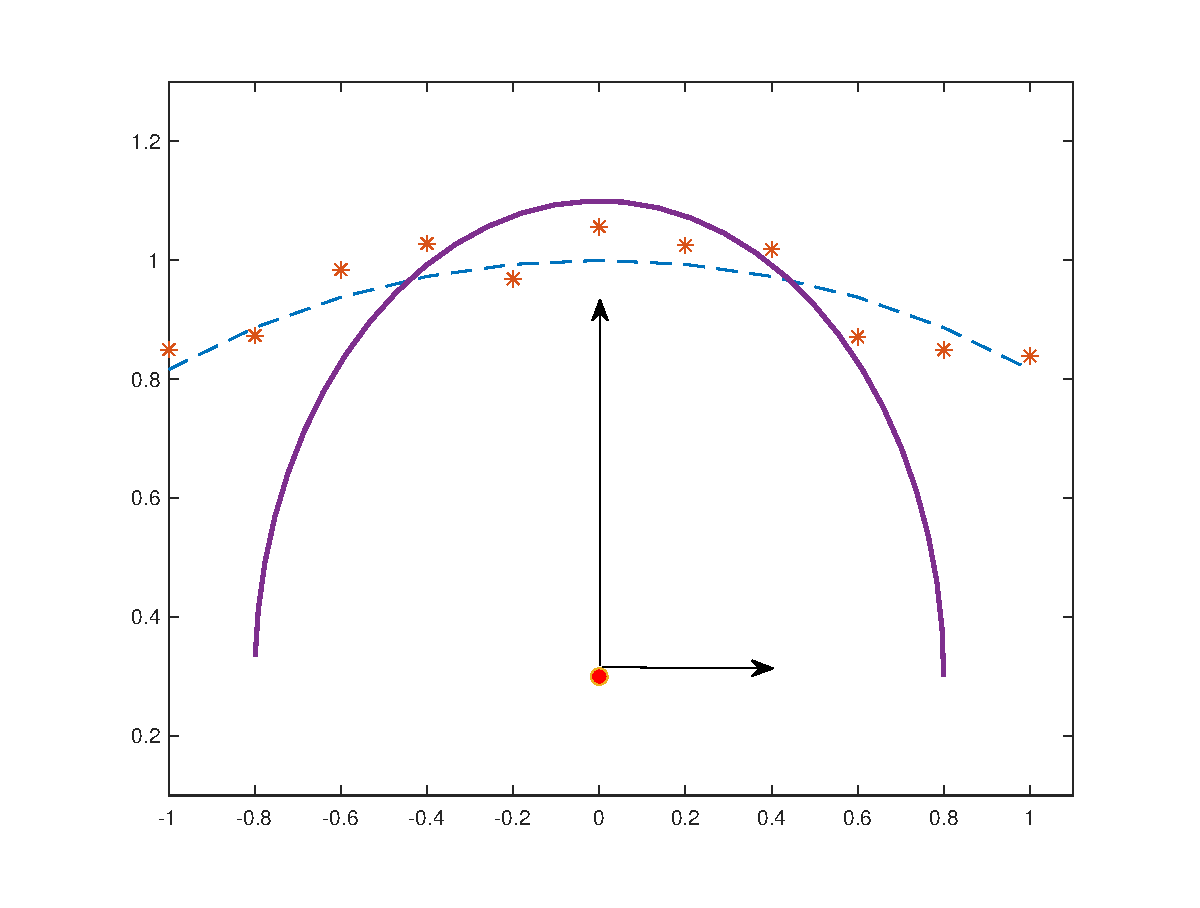
\includegraphics[width=0.32\linewidth]{../figures/demo1.eps} 
%\hspace{-4mm}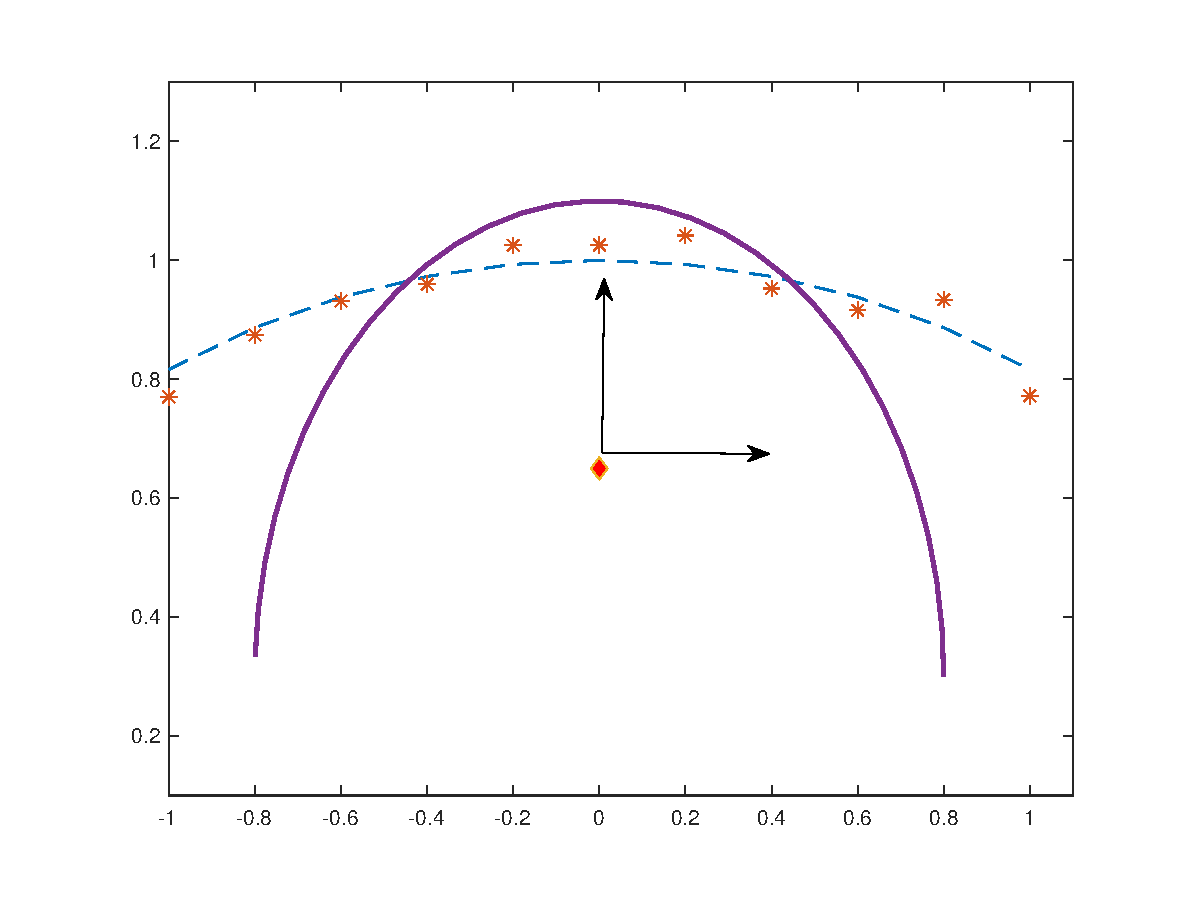
\includegraphics[width=0.32\linewidth]{../figures/demo2.eps} 
%\hspace{-4mm}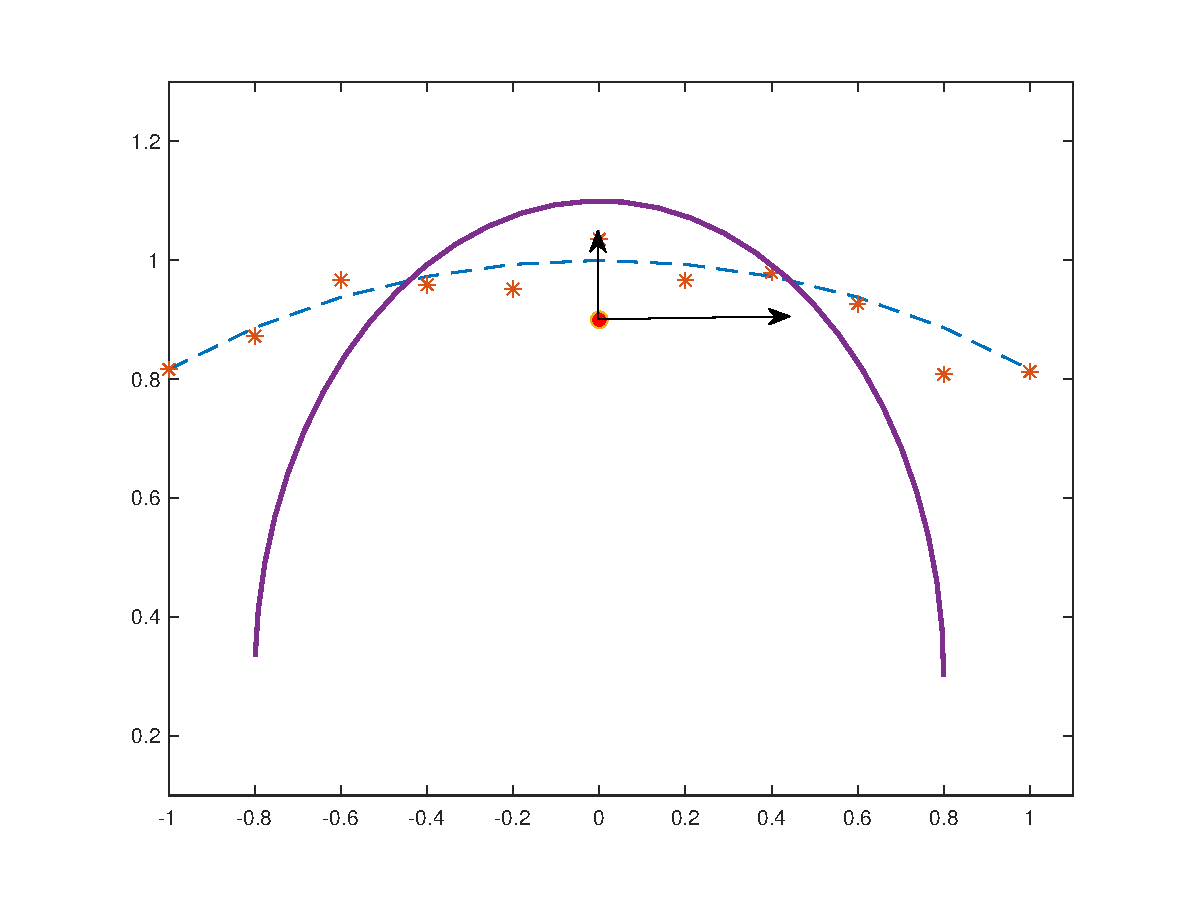
\includegraphics[width=0.32\linewidth]{../figures/demo3.eps} 
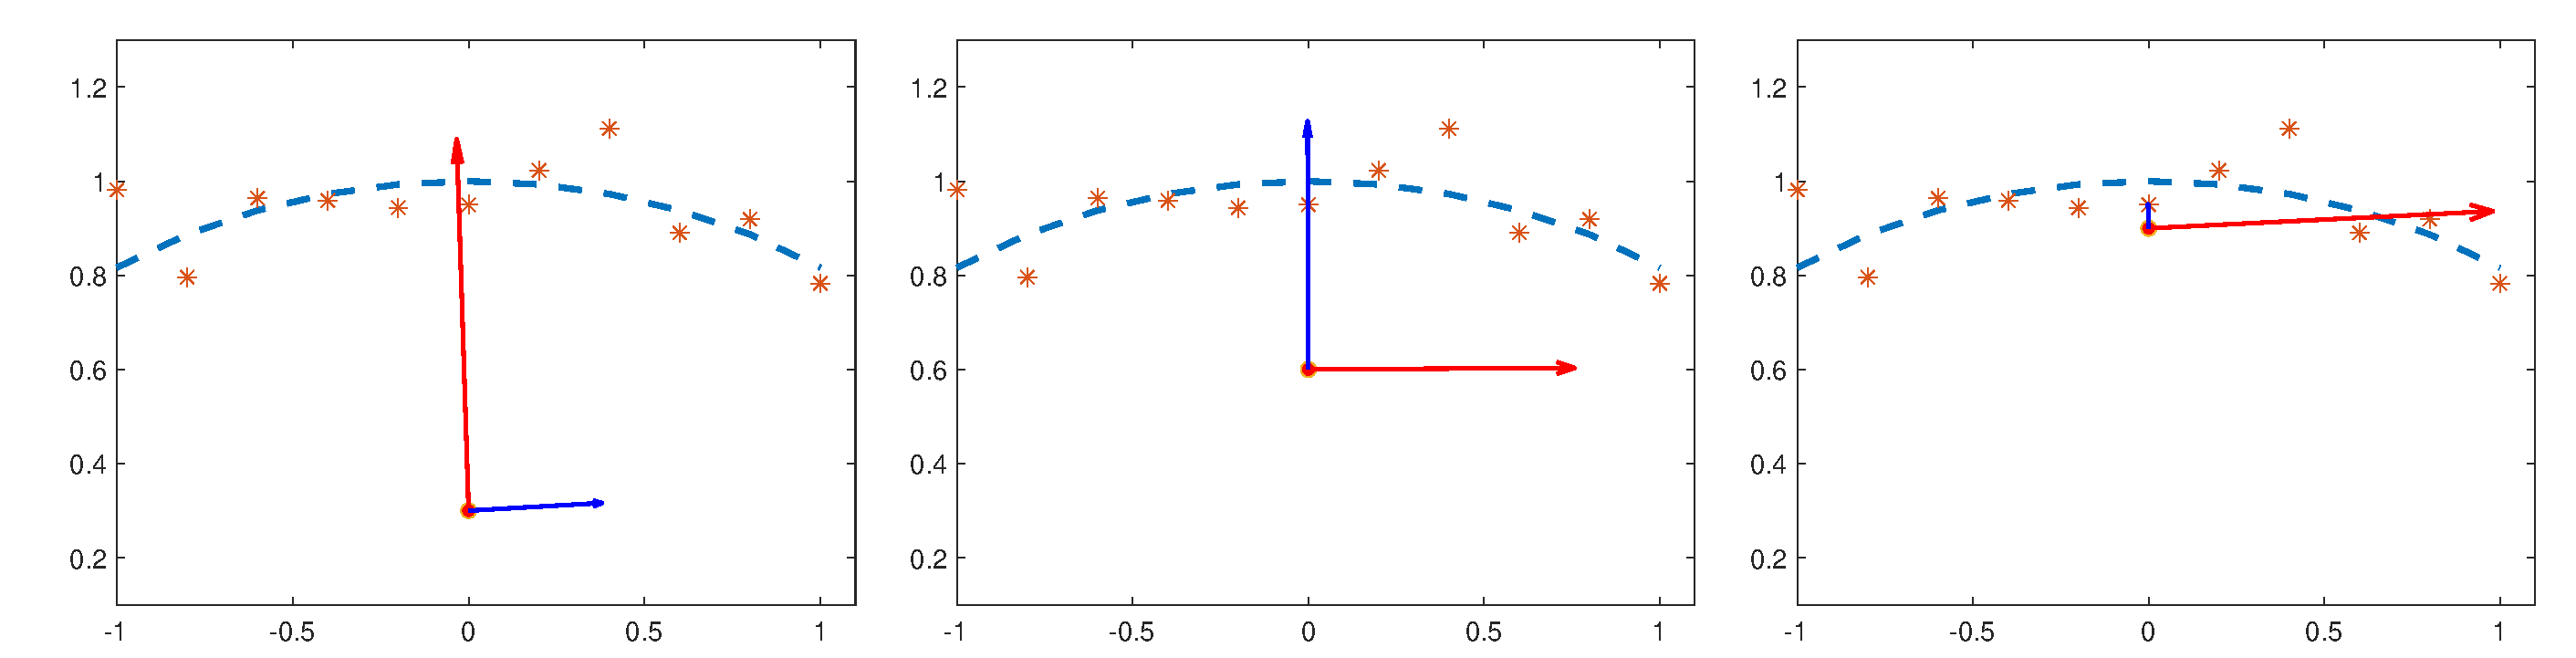
\includegraphics[width=\linewidth]{demo123.eps} 
%\setcaptionwidth{6in}
\caption{The process of $J_r(x)$'s eigenspace's variation with $x$ approaching the manifold }
\label{Shifting Eigenvectors}
\end{figure}

\subsubsection*{Case \romannumeral1: $\lambda(A(x))>\lambda_{\max} (\Xi(x))$}

This case corresponds to the leftmost diagram in {Figure \ref{Shifting Eigenvectors}}, where $x$ is far away from the data points. The covariance matrix $\sum_i w_h(x_i, x)(x_i-x)(x_i-x)^T$ will have large eigenvalues in the subspace of $V_{D-d}(C_r(x))$. Then, the eigenvector $V_{D-d}(C_r(x))\alpha(x)$ is the principal eigenvector, and we can distinguish it from the top eigenvector through eigenvalue decomposition.
Then, the eigen-decomposition of $J_r(x)$ is
\begin{equation}\label{SVD1}
J_r (x)= [v(x), \Upsilon(x)] 
\left[
\begin{array}{cc}
\lambda(A(x)) & \bf 0\\
\bf 0 &\Lambda(x)
\end{array}
\right][v(x), \Upsilon(x)]^T.
\end{equation}
From \eqref{SVD1}, we can recover the space spanned by $V_{D-d}(c_r(x))\alpha(x)$ by choosing the eigenvectors corresponding to the largest eigenvector. The space corresponding to $V_d(c_r(x))$ can be recovered by choosing the 2nd to $(d+1)$-th eigenvectors of $J_r(x)$.

\subsubsection*{Case \romannumeral2: $\lambda_{\min} (\Xi(x)) \leq \lambda(A(x))\leq \lambda_{\max} (\Xi(x))$}

This case corresponds to the middle figure in {Figure \ref{Shifting Eigenvectors}}, where $x$ is in the middle range of distance from the data points. In this case, the eigenvalue corresponding to $V_{D-d}(C_r(x))\alpha(x)$ is disguised by the eigenvalues of $B(x)$. Here, we cannot distinguish the eigenspace of $V_{D-d}(C_r(x))\alpha(x)$ by simply choosing the eigenvector corresponding to the largest or the smallest eigenvalue. The eigen-decomposition of $J(x)$ yields the following form:
\begin{equation}\label{SVD2}
J_r (x)= [\Upsilon_1(x), v(x), \Upsilon_2(x)] 
\left[
\begin{array}{ccc}
\Lambda_1(x) & \bf 0 & \bf 0\\
\bf 0 &\lambda(A(x)) &\bf 0 \\
\bf 0 &\bf 0  &\Lambda_2(x) \\
\end{array}
\right][\Upsilon_1(x), v(x), \Upsilon_2(x)]^T,
\end{equation}
where each diagonal element of $\Lambda_1(x)$ is greater than $\lambda(A(x))$, and each diagonal element of $\Lambda_2(x)$ is less than $\lambda(A(x))$.

For {\it Case {\romannumeral1}} and {\it Case \romannumeral2},  the d-dimensional projection $P(J_r(x))$ corresponding to the eigenspaces of $J_r(x)$ is different with that of $C_r(x)$. The error of the two projections is
\[
P(J_r(x)) - P(C_r(x)) = v v^T - u_du_d^T,
\]
where $u_d$ is the eigenvector corresponding to the $d$-th largest eigenvalue of $B(x)$. Clearly, we have the operator norm
\[
\| P(J_r(x)) - P(C_r(x)) \|_2 = 1.
\]

\subsubsection*{Case \romannumeral3: $\lambda(A(x))<\lambda_{\min} (\Xi(x))$ }

This case corresponds to the rightmost diagram in {Figure \ref{Shifting Eigenvectors}}, where $x$ is in a small range of distance from the data points. The covariance matrix $\sum_i w_h(x_i, x)(x_i-x)(x_i-x)^T$ will have large eigenvalues corresponding to the eigenvectors parallel with the tangent space at $c_r(x)$. Then, the variance along $V_{D-d}(x)\alpha(x)$ will become relatively small, causing the eigen-decomposition form of $J(x)$ to yield the following form:
\begin{equation}\label{SVD3}
J_r (x)= [\Upsilon(x),v(x)] 
\left[
\begin{array}{cc}
\Lambda(x) & \bf 0\\
\bf 0 &\lambda(A(x))
\end{array}
\right][\Upsilon(x), v(x)]^T.
\end{equation}
In this case, to recover $V_d(C_r(x))$, we can simply choose the eigenvectors corresponding to the top $d$ eigenvalues of $\sum_i w_h(x_i, x)(x_i-x)(x_i-x)^T$. As a result, we can replace $C_r(x)$ by $J_r(x)$ to compute the space $V_d(C_r(x))$.

For {\it Case {\romannumeral3}},  the d-dimensional projection $P(J_r(x))$ corresponding to the eigenspaces of $J_r(x)$ is the same with that of $C_r(x)$. Thus, the error of the two projections is
\[
P(J_r(x)) - P(C_r(x)) = 0,
\]
and the operator norm $\|P(J_r(x)) - P(C_r(x))\|_2=0$.
%\begin{remark}

%Based on the analysis, we know that we cannot simply use the eigenspace of $J_r(x)$ instead of $C_r(x)$ in any occasion. Below, we will show how the existing difference in the behaviors of eigenspace influence our ridges, respectively.
%\end{remark}
\end{proof}

\section{}
\subsection{Rank-one Modification Enlarges Projection}
\begin{lemma}
{ For any symmetric matrix $B$, let $A = B +\lambda uu^T, \forall \lambda\geq 0$. We  have $\|\Pi_A u\|_2\geq \|\Pi_B u\|_2$, where $\Pi_A, \Pi_B$ are the projections onto the space spanned by the eigenvectors corresponding to the $d$ largest eigenvalues of $A$ and $B$, respectively.}
\label{projection_enlarge}
\end{lemma}


\begin{proof}\label{Rank-one Enlarge Projection}
Because of the variational inequality of eigenvectors, the top $d$ eigenvectors can be written as the solution of the maximum optimal problem
 \[
 \begin{aligned}
U_A = \arg\max_{U^TU = I_d} {\rm trace} (U^T A U),\\
U_B = \arg\max_{U^TU = I_d} {\rm trace} (U^T B U).
\end{aligned}
\]
Denote $\Pi_A = U_A {U_A}^T,  \Pi_B = U_B {U_B}^T$. Because for any $Z$ and $W$ with the same shape, the trace and inner product is equal  by 
\[
{\rm trace} (Z^TW) = \langle Z, W\rangle.
\]
where the inner product of two matrices with the same shape is defined as:
$
\langle Z,W \rangle = \sum_{ij} Z_{ij} W_{ij}
$
Therefore, we have:
\[
{\rm trace} (U_A^T A U_A) = {\rm trace} (U_A U_A^T A ) =\langle U_AU_A^T, A\rangle = \langle  \Pi_A, A\rangle.
\]
Similarly, 
\[
{\rm trace} (U_B^T B U_B) = {\rm trace} (U_B U_B^T B ) =\langle U_BU_B^T, B\rangle = \langle  \Pi_B, B\rangle.
\]
Using variational results about eigenvalues on $A$ and $B$, we have 
\begin{equation}\label{variantional}
\langle \Pi_B , B \rangle \geq \langle \Pi_A , B \rangle,  \quad \langle \Pi_A , A \rangle \geq \langle \Pi_B , A \rangle.
\end{equation}
For the definition of the inner product $\langle \cdot, \cdot \rangle$ of two matrices with the same shape, please refer to the footnote. Because of $\langle \Pi_B , B \rangle \geq \langle \Pi_A , B \rangle$, we have
\begin{equation}\label{temp2}
\langle \Pi_B, B\rangle+ \langle \Pi_A, \lambda uu^T\rangle \leq \langle \Pi_A, B+\lambda uu^T \rangle.
\end{equation}
Recalling the definition of $A$, the right side of \eqref{temp2} equals to
\begin{equation}\label{temp3}
\langle \Pi_A, B+\lambda uu^T \rangle = \langle \Pi_A , A \rangle.
\end{equation}
Using variational results about eigenvalues of $A$, we have:
\begin{equation}\label{temp4}
\langle \Pi_A , A \rangle \geq  \langle \Pi_B, B+\lambda uu^T \rangle=\langle \Pi_B, B\rangle + \langle \Pi_B, \lambda uu^T \rangle.
\end{equation}
Combining \eqref{temp2}, \eqref{temp3}, \eqref{temp4} and
%\[
%\begin{aligned}
%&\langle \Pi_B, B\rangle+ \langle \Pi_A, \lambda uu^T\rangle\\
% \geq &\langle \Pi_A, B+\lambda uu^T \rangle = \langle \Pi_A , A \rangle   \geq  \langle \Pi_B, B+\lambda uu^T \rangle =  \langle \Pi_B, B\rangle + \langle \Pi_B, \lambda uu^T \rangle.
%\end{aligned}
%\]
eliminating the term $\langle \Pi_B, B\rangle$, we have:
\begin{equation}\label{step1}
\langle  \Pi_A , uu^T\rangle \geq  \langle  \Pi_B,  uu^T\rangle.
\end{equation}
Because of
\begin{equation}\label{step2}
\langle \Pi_A, uu^T \rangle= u^T \Pi_A u = u^T \Pi_A \Pi_A u = \|\Pi_A u\|_2^2,
\end{equation}
Using \eqref{step1} and \eqref{step2}, we will achieve that $\|\Pi_A u\|_2\geq \|\Pi_B u\|_2$.
\end{proof}
\subsection{Rank-one Modification on Subspace}
\begin{lemma}\label{eigvenvalue}
For any symmetric matrix $B$, let $A = B+\lambda u u^T$,  $\forall \lambda \geq 0$ and any nonzero vector $u\in  {\rm span}\{ u_1(B(x)), u_2(B(x)),..., u_d(B(x))\}$, the $(d+1)$-th  to $D$-th largest eigenvalues of $A$ and $B$ yields, 
\[
\lambda_{d+k}(A) = \lambda_{d+k}(B),\quad k=1,...,D-d
\]
%where ${\cal S}_d = {\rm span}\{ u_1(B(x)), u_2(B(x)),..., u_d(B(x))\}$
where $u_k(B(x))$ and $\lambda_k(B(x))$ are the eigenvector and eigenvalue corresponding to the $k$-th largest eigenvalues of $B(x)$\end{lemma}
\begin{proof}
We use $\Lambda^{(1)}, \Lambda^{(2)}$ to stand for the $d\times d$ and $(n-d)\times(n-d)$ diagonal matrix corresponding the eigenvalue decomposition of $B$. Denote the eigenvalue decomposition of $B$ as
\[
B = [U_d, U_{n-d}] 
\left[
\begin{array}{cc}
\Lambda^{(1)} &\\
 &\Lambda^{(2)}
\end{array}
\right]
[U_d, U_{n-d}]^T.
\]
Since $u\in {\cal S}_d$, we can write $u$ by the combination of the columns of $U_d$ as $u = U_d\alpha$, then,
\[
B+\lambda u u^T = [U_d, U_{n-d}] 
\left[
\begin{array}{cc}
\Lambda^{(1)} &\\
  &\Lambda^{(2)}
\end{array}
\right]
[U_d, U_{n-d}]^T+ \lambda U_d \alpha \alpha^T U_d^T.
\]
Denote the eigenvalue decomposition of as
\[
U_d\Lambda^{(1)} U_d^T+\lambda U_d \alpha \alpha^T U_d^T = \hat{U}_d {\Lambda} \hat{U}_d^T,
\]
where the diagonal elements in $\Lambda, \Lambda^{(1)}$ are placed in decreasing order. By the Weyl's theorem for eigenvalues \cite{horn2012matrix}, we know 
\[
{\Lambda}_{ii}\geq {\Lambda}_{ii}^{(1)}, \quad i=1,..., d.
\] 
and
\[
{\Lambda}_{ii}\geq {\Lambda}_{ii}^{(1)}\geq {\Lambda}_{jj}^{(2)},  \forall, i=1,..., d, \forall, j= 1,...,D-d.
\] 
Thus, the eigenvalue decomposition of $A$ is
\[
A = [\hat{U}_d, U_{n-d}] 
\left[
\begin{array}{cc}
\Lambda & \\
 & \Lambda^{(2)}
\end{array}
\right]
[\hat{U}_d, U_{n-d}]^T.
\]
Note that, because the columns of $U_d$ and $\hat{U}_d$ span the same subspace and the columns of $U_d$ is orthogonal with the columns of $U_{n-d}$, we know that the columns of $\hat{U}_d$ is also orthogonal with the columns of $U_{n-d}$.

Because of the uniqueness of the eigenvalue decomposition, we have proved that 
\[
\lambda_{d+1}(A) = \lambda_{d+1}(B) = \Lambda^{(2)}_{1 1}.
\]
Furthermore, for the remaining eigenvalues, we have the similar result as
\[
\lambda_{d+k}(A) = \lambda_{d+k}(B) = \Lambda^{(2)}_{k k}\quad \forall, k = 1,...,D-d.
\]
\end{proof}
%\remark{
%
%}
\subsection{Inclusion Lemma}
%Define $R_\ell(f(p))$ to be the set:
%\[
% \{x | \Pi_{H_{f(p)}}^{\perp} (x) \nabla f(p(x)) = 0,\lambda_{d+1}(H_{f(p)}(x))<  {f''(p(x))}\|\nabla p(x)\|_2^2\}.
%\]
%\remark{
%Since ${f''(p(x))}\leq 0$, the condition for $R_\ell(f(p))$ is stronger than $R(f(p))$, thus $R_\ell(f(p))$ is part of $R(f(p))$.
%}
\begin{lemma}{
For any monotonously increasing and concave function $f(y)$, i.e,  $f'(x)>0, f''(x) \leq 0$, for $x\in R({f(p)})$, then, we have the following satisfied simultaneously:
 \begin{gather*}
 \lambda_{d+1}(H_p(x)) < 0,\\
\|\Pi_{H_p}^\perp(x)\nabla p(x)\|_2 \leq \|\Pi_{H_{f(p)}}^{\perp}(x)\nabla p(x)\|_2=0,
%\frac{1}{f'(p(x))}( \lambda_{d+1} (H_{f(p)}(x))-{f''(p(x))}\|\nabla p(x)\|_2^2)\leq 0
\end{gather*}
the condition $\|\Pi_{H_p}^\perp(x)\nabla p(x)\|_2  =0$ implies $\Pi_{H_p}^\perp(x)\nabla p(x)=\bf 0$ which indicates that $x\in R(p)$. Thus, $R(f(p)) \subset R(p)$}. %where $p(x)$ is a twice-differentiable density function. 
%\label{rankonetheorem}
\label{monotonously theorem} 
\end{lemma}

\begin{proof}\label{monotonously theorem proof}
Recall that $H_p(x)$ is a rank-one modification with $H_{f}(x)$ by 
\begin{equation}\label{rankone}
 H_{p}(x) =\frac{1}{ f'(p(x))} H_{f(p)}(x) - \frac{f''(p(x))}{ f'(p(x))} \nabla p(x) \nabla^T p(x) .
\end{equation}
 Because $f(y)$ is a monotonously increasing and concave function, we know 
\[
- f''(p(x))/f'(p(x))>0.
\] 
Thus, $H_{p}(x)$ is obtained from a nonnegative rank-one modification. Lemma \ref{projection_enlarge} implies
\begin{equation}\label{enlargement}
\|\Pi_{H_p}(x)\nabla p(x)\|_2 \geq \|\Pi_{H_{f(p)}}(x)\nabla p(x)\|_2.
\end{equation}
where the projection matrix $\Pi_{H_p}$ and $\Pi_{H_{f_p}} $ defined as
\[
\begin{aligned}
&\Pi_{H_p}(x)= U_d(H_p(x))U^T_d(H_p(x)), \\
&\Pi_{H_{f_p}}(x) = U_d(H_{f(p)}(x))U^T_d(H_{f_p}(x)),
\end{aligned}
\]
Here, $U_d(H_p(x))$and $U^T_d(H_p(x))$ are the eigenvectors corresponding to the largest $d$ eigenvalues of $H_p(x)$ and $H_{f_p}(x)$, respectively.
%\[
%\|\Pi_{H_p}^\perp(x)\nabla p(x)\|_2 \leq \|\Pi_{H_{f(p)}}^{\perp}(x)\nabla p(x)\|_2
%\]

For any two projections $\Pi_{H_p}(x), \Pi_{H_{f(p)}}(x)$ and their orthogonal complement projection $\Pi^\perp_{H_p}(x), \Pi^\perp_{H_{f(p)}}(x)$, because of the orthogonal properties with respect to $\Pi_{H_p}^{\perp}(x)$ and $\Pi_{H_p}(x)$ , we have the following two equalities:
\begin{equation}\label{ortho1}
\|\Pi_{H_p}^{\perp}(x) \nabla p(x)\|_2^2 +\|\Pi_{H_p}(x) \nabla p(x)\|_2^2 = \|\nabla p(x)\|_2^2.
\end{equation}
Similarly, for $\Pi_{H_{f(p)}}^{\perp}(x)$ and $\Pi_{H_{f(p)}}(x)$, because of the orthogonal properties, there is
\begin{equation}\label{ortho2}
\|\Pi_{H_{f(p)}}^{\perp}(x) \nabla p(x)\|_2^2 +\|\Pi_{H_{f(p)}}(x) \nabla p(x)\|_2^2 = \|\nabla p(x)\|_2^2.
\end{equation}
Because of \eqref{ortho1} and \eqref{ortho2}, we know that the condition (squaring both sides in \eqref{enlargement})
 \[
\|\Pi_{H_p}(x)\nabla p(x)\|_2^2 \geq \|\Pi_{H_{f(p)}}(x)\nabla p(x)\|_2^2,
\] 
implies
\begin{equation}\label{square_result}
\|\Pi_{H_p}^{\perp}(x)\nabla p(x)\|_2^2 \leq \|\Pi_{H_{f(p)}}^{\perp}(x)\nabla p(x)\|_2^2.
\end{equation}
Taking the square root of both sides in \eqref{square_result} will lead to
\begin{equation}\label{llll}
\|\Pi_{H_p}^{\perp}(x)\nabla p(x)\|_2 \leq \|\Pi_{H_{f(p)}}^{\perp}(x)\nabla p(x)\|_2.
\end{equation}
%To prove $\|\Pi_{H_p}(x)\nabla p(x)\|_2 \geq \|\Pi_{H_{f(p)}}(x)\nabla p(x)\|_2$ is equivalent to prove 
%\begin{equation}\label{relationHF}
%\nabla p(x)^T \Pi_{H_p}(x) \nabla p(x)\geq \nabla p(x)^T \Pi_{H_{f(p)}}(x) \nabla p(x),
%\end{equation} 
%which is clear, as the $d$ principal components of $H_p(x)$ are enlarged by adding a rank-one modification in the direction of $\nabla p(x)\nabla p(x)^T$ from $H_f(x)$; this is proved in Lemma \ref{projection_enlarge}.
It is easy to obtain $\Pi_{H_{f(p)}}^{\perp}(x)\nabla p(x) = 0$. For any $x\in R_{f(p(x))}$, use the definition of ridge, we have 
\[
 \Pi_{H_{f(p)}}^{\perp} (x) \nabla p(x) = 0,\quad \lambda_{d+1}(H_{f(p)}(x))<0
\] %i.e., $\nabla p(x)\perp {\rm span}\{ u^{d+1}_{H_f}(x), ...,u^{D}_{H_f}(x)\}$; 
%in other words, \[
%\nabla p(x)\in {\rm span}\{u^{1}_{H_f}(x), ..., u^{d}_{H_f}(x) \}.
%\] 
Because of $\|\Pi_{H_p}^\perp(x)\nabla p(x)\|_2 \leq \|\Pi_{H_{f(p)}}^{\perp}(x)\nabla p(x)\|_2$, we have 
\[
\|\Pi_{H_{f(p)}}^{\perp}(x)\nabla p(x)\|_2=0
\] 
implies that we also have $\|\Pi_{H_p}^\perp(x)\nabla p(x)\|_2=0$. Next, we show $\lambda_{d+1}(H_p(x)) < 0$. Recall that, 
\[
 H_{p}(x) =\frac{1}{ f'(p(x))} H_{f(p)}(x) - \frac{f''(p(x))}{ f'(p(x))} \nabla p(x) \nabla^T p(x) .
\]
%Recall  in \eqref{rankone} is equivalent to
%\[
% H_{f(p)}(x) = f'(p(x))\{ H_{p}(x)+ \frac{f''(p(x))}{f'(p(x))} \nabla p(x) \nabla^T p(x) \}  .
%\]
 Thus, $-{f''(p(x))} \nabla p(x) \nabla^T p(x)$ is a semi-positive definite modification.
 Because $\|\Pi_{H_p}^\perp(x)\nabla p(x)\|_2=0$,  which implies $\nabla p(x)$ is in the space spanned by
 \[
 {\cal S}_{H_{f(p)}(x)} = {\rm span}\{ u_1(H_{f(p)}(x)), u_2(H_{f(p)}(x)),..., u_d(H_{f(p)}(x))\}
 \]
 Because $\nabla p(x) \in  {\cal S}_{H_{f(p)}(x)}$,  the semi-positive rank-one modification
 \[
 -{f''(p(x))} \nabla p(x) \nabla^T p(x)
 \] 
 on the matrix $H_{f(p)}(x)$ is equivalent to rank-one modification on the principal $d$-dimensional subspace ${\cal S}_{H_{f(p)}(x)}$ which will not affect the orthogonal complement subspace ${\cal S}^\perp_{H_{f(p)}(x)}$, which means the
 eigenvalues from the $(d+1)$-th largest eigenvalue to $D$-th will keep unchanged by Lemma \eqref{eigvenvalue}. % \cite{horn2012matrix}.
%Using the Weyl's theorem \cite{horn2012matrix} on eigenvalues, 
Thus, we have :
\[
\lambda_{d+1}(H_p(x))  = \frac{1}{f'(p(x))} \lambda_{d+1}(H_{f(p)}(x)) < 0, %\frac{1}{ f'(p(x))}(\lambda_{d+1}(H_{f(p)}(x))- {f''(p(x))} \lambda(\nabla p(x) \nabla^T p(x)))
\]
because of $f'(p(x))>0$ and ${f''(p(x))}<0$. %We know that,
%\[
%\lambda_{d+1}(H_{f(p)}(x)) \leq {f''(p(x))}\|\nabla p(x)\|_2^2,
%\]
%is equvilant to
%\[
%\lambda_{d+1}(H_p(x)) \leq 0.
%\]
In conclusion, $x$ also satisfies the ridge condition derived by $p(x)$, i.e. $x \in R({p(x)})$, which implies $R({f(p(x))}) \subset R({p(x)})$. 

%We can conclude that, as long as $\nabla p(x)$ is in the space spanned by the top $d$ eigenvectors of $H_{f(p)}(x)$, $\nabla p(x)$ is in the space spanned by the top $d$ eigenvectors of $H_p(x)$, i.e. $\Pi_{H_p}^{\perp}(x) \nabla p(x) = 0$, which means $x \in R_{p(x)}$. Thus, we can conclude that $R_{f(p(x))} \subset R_{p(x)}$. 

\end{proof}
\subsection{Transformed Inequality}
\begin{theorem}\label{Transformed Inequality Theorem}
For the ridge $R(f(p))$ defined by the transformed nonlinear increasing and concave function $f$, we have:
\[
{\rm Haus} (R(f(p)), {\cal M}_{R(f(p))}) \leq {\rm Haus} (R(p), {\cal M}_{R(p)}),
\]
where $R(p)$ and $R(f(p))$ are the $d$-dimensional ridges corresponding to $p$ and $f(p)$, ${\cal M}_{R(p)}$ and ${\cal M}_{R(f(p))}$ are the projections of $R(p)$ and $R(f(p))$ onto $\cal M$, respectively.
%$\sup_{x\in R_f} \inf_{y\in {\cal M}_R} \|x-y\|_2 \leq {\rm Haus} (R, {\cal M}_{R})$
\end{theorem}

\begin{proof}\label{Transformed Inequality}
Since the projection from $R$ to ${\cal M}_{R}$ is surjective, for any $y^*\in {\cal M}_{R}$, such as
$\inf_{x\in R} \|x-y^*\| = \sup_{y\in {\cal M}_R} \inf_{x\in R}\|x-y\|_2$, there is $x_{y^*}\in R$ such as $y = P_{{\cal M}_R}(x_{y^*})$. 
\[
\begin{aligned}
&\sup_{y\in {\cal M}_R} \inf_{x\in R}\|x-y\|_2 \\
=&\inf_{x\in R} \|x-y^*\|_2 \leq \|x_{y^*} - y^*\|_2 \\
= &\inf_{z\in{\cal M}_R }\|x_{y^*}-z\|_2 \leq \sup_{x\in R}\inf_{z\in{\cal M}_R }\|x-z\|_2.
\end{aligned}
\]
%Therefore, we have $\sup_{x\in {R}} \inf_{y\in {\cal M}_R}\|x-y\|_2\geq  \sup_{y\in {\cal M}_R} \inf_{x\in R}\|x-y\|_2$
Since ${\rm Haus} (R, {\cal M}_{R}) = \max \{\sup_{x\in R} \inf_{y\in {\cal M}_R} \|x-y\|_2, \sup_{x\in {\cal M}_R} \inf_{y\in R} \|x-y\|_2\}$, we can conclude that
\[
{\rm Haus} (R, {\cal M}_{R}) = \sup_{x\in R} \inf_{y\in {\cal M}_R} \|x-y\|_2.
\]
Also, noting that $R = R/R_f\cup R_f$, we know that
\begin{equation}\label{partial_ridge}
\sup_{x\in R} \inf_{y\in {\cal M}_R} \|x-y\|_2 = \max\{\sup_{x\in R/R_f} \inf_{y\in {\cal M}_R} \|x-y\|_2, \sup_{x\in R_f} \inf_{y\in {\cal M}_R} \|x-y\|_2 \}.
\end{equation}
Because of \eqref{partial_ridge}, we can easily obtain
\begin{equation}\label{m_R_f_1}
\sup_{x\in R_f} \inf_{y\in {\cal M}_R} \|x-y\|_2 \leq {\rm Haus} (R, {\cal M}_{R}).
\end{equation}
Because of $R_f\subset R$, thus, we have ${\cal M}_{R_f}\subset {\cal M}_R$.  Also, notice that ${\cal M}_{R_f}$ is the projection on $R_f$ onto $\cal M$ and ${\cal M}_R$ is the projection of $R$ onto $\cal M$. We have
\begin{equation}\label{m_R_f_2}
\sup_{x\in R_f} \inf_{y\in {\cal M}_{R_f}} \|x-y\|_2=\sup_{x\in R_f} \inf_{y\in {\cal M}_R} \|x-y\|_2.
\end{equation}
The projection from $R_f$ to ${\cal M}_{R_f}$ is surjective, which implies the Hausdorff distance equals the quasi-Hausdorff, \cite{chen2015asymptotic} i.e., 
\begin{equation}\label{m_R_f_3}
{\rm Haus} (R_f, {\cal M}_{R_f}) = \sup_{x\in R_f} \inf_{y\in {\cal M}_{R_f}} \|x-y\|_2,
\end{equation}
Combining \eqref{m_R_f_1},\eqref{m_R_f_2},\eqref{m_R_f_3}, we have:
$
{\rm Haus} (R_f, {\cal M}_{R_f}) \leq {\rm Haus} (R, {\cal M}_{R}).
$
\end{proof}

\end{appendix}



%\bibliographystyle{imsart-number}
\bibliographystyle{imsart-nameyear}
\bibliography{bibfile}


\end{document}

This template helps you to create a properly formatted \LaTeXe\ manuscript.
%%%%%%%%%%%%%%%%%%%%%%%%%%%%%%%%%%%%%%%%%%%%%%
%% `\ ' is used here because TeX ignores    %%
%% spaces after text commands.              %%
%%%%%%%%%%%%%%%%%%%%%%%%%%%%%%%%%%%%%%%%%%%%%%
Prepare your paper in the same style as used in this sample .pdf file.
Try to avoid excessive use of italics and bold face.
Please do not use any \LaTeXe\ or \TeX\ commands that affect the layout
or formatting of your document (i.e., commands like \verb|\textheight|,
\verb|\textwidth|, etc.).

\section{Section headings}
Here are some sub-sections:
\subsection{A sub-section}
Regular text.
\subsubsection{A sub-sub-section}
Regular text.

\section{Text}
\subsection{Lists}

The following is an example of an \emph{itemized} list,
two levels deep.
\begin{itemize}
\item
This is the first item of an itemized list.  Each item
in the list is marked with a ``tick.''  The document
style determines what kind of tick mark is used.
\item
This is the second item of the list.  It contains another
list nested inside it.
\begin{itemize}
\item This is the first item of an itemized list that
is nested within the itemized list.
\item This is the second item of the inner list.  \LaTeX\
allows you to nest lists deeper than you really should.
\end{itemize}
This is the rest of the second item of the outer list.
\item
This is the third item of the list.
\end{itemize}

The following is an example of an \emph{enumerated} list of one level.

\begin{longlist}
\item This is the first item of an enumerated list.
\item This is the second item of an enumerated list.
\end{longlist}

The following is an example of an \emph{enumerated} list, two levels deep.
\begin{longlist}
\item[1.]
This is the first item of an enumerated list.  Each item
in the list is marked with a ``tick.''  The document
style determines what kind of tick mark is used.
\item[2.]
This is the second item of the list.  It contains another
list nested inside of it.
\begin{longlist}
\item
This is the first item of an enumerated list that
is nested within.  
\item
This is the second item of the inner list.  \LaTeX\
allows you to nest lists deeper than you really should.
\end{longlist}
This is the rest of the second item of the outer list.
\item[3.]
This is the third item of the list.
\end{longlist}

\subsection{Punctuation}
Dashes come in three sizes: a hyphen, an intra-word dash like ``$U$-statistics'' or ``the time-homogeneous model'';
a medium dash (also called an ``en-dash'') for number ranges or between two equal entities like ``1--2'' or ``Cauchy--Schwarz inequality'';
and a punctuation dash (also called an ``em-dash'') in place of a comma, semicolon,
colon or parentheses---like this.

Generating an ellipsis \ldots\ with the right spacing
around the periods requires a special command.

\section{Fonts}
Please use text fonts in text mode, e.g.:
\begin{itemize}
\item[]\textrm{Roman}
\item[]\textit{Italic}
\item[]\textbf{Bold}
\item[]\textsc{Small Caps}
\item[]\textsf{Sans serif}
\item[]\texttt{Typewriter}
\end{itemize}
Please use mathematical fonts in mathematical mode, e.g.:
\begin{itemize}
\item[] $\mathrm{ABCabc123}$
\item[] $\mathit{ABCabc123}$
\item[] $\mathbf{ABCabc123}$
\item[] $\boldsymbol{ABCabc123\alpha\beta\gamma}$
\item[] $\mathcal{ABC}$
\item[] $\mathbb{ABC}$
\item[] $\mathsf{ABCabc123}$
\item[] $\mathtt{ABCabc123}$
\item[] $\mathfrak{ABCabc123}$
\end{itemize}
Note that \verb|\mathcal, \mathbb| belongs to capital letters-only font typefaces.

\section{Notes}
Footnotes\footnote{This is an example of a footnote.}
pose no problem.\footnote{Note that footnote number is after punctuation.}

\section{Quotations}

Text is displayed by indenting it from the left margin. There are short quotations
\begin{quote}
This is a short quotation.  It consists of a
single paragraph of text.  There is no paragraph
indentation.
\end{quote}
and longer ones.
\begin{quotation}
This is a longer quotation.  It consists of two paragraphs
of text.  The beginning of each paragraph is indicated
by an extra indentation.

This is the second paragraph of the quotation.  It is just
as dull as the first paragraph.
\end{quotation}

\section{Environments}

\subsection{Examples for \emph{\texttt{plain}}-style environments}
\begin{axiom}\label{ax1}
This is the body of Axiom \ref{ax1}.
\end{axiom}

\begin{proof}
This is the body of the proof of the axiom above.
\end{proof}

\begin{claim}\label{cl1}
This is the body of Claim \ref{cl1}. Claim \ref{cl1} is numbered after
Axiom \ref{ax1} because we used \verb|[axiom]| in \verb|\newtheorem|.
\end{claim}

\begin{theorem}\label{th1}
This is the body of Theorem \ref{th1}. Theorem \ref{th1} numbering is
dependent on section because we used \verb|[section]| after \verb|\newtheorem|.
\end{theorem}

\begin{theorem}[Title of the theorem]\label{th2}
This is the body of Theorem \ref{th2}. Theorem \ref{th2} has additional title.
\end{theorem}

\begin{lemma}\label{le1}
This is the body of Lemma \ref{le1}. Lemma \ref{le1} is numbered after
Theorem \ref{th2} because we used \verb|[theorem]| in \verb|\newtheorem|.
\end{lemma}


\begin{proof}[Proof of Lemma \ref{le1}]
This is the body of the proof of Lemma \ref{le1}.
\end{proof}

\subsection{Examples for \emph{\texttt{remark}}-style environments}
\begin{definition}\label{de1}
This is the body of Definition \ref{de1}. Definition \ref{de1} is numbered after
Lemma \ref{le1} because we used \verb|[theorem]| in \verb|\newtheorem|.
\end{definition}

\begin{example}
This is the body of the example. Example is unnumbered because we used \verb|\newtheorem*|
instead of \verb|\newtheorem|.
\end{example}

\begin{fact}
This is the body of the fact. Fact is unnumbered because we used \verb|\newtheorem*|
instead of \verb|\newtheorem|.
\end{fact}

\section{Tables and figures}
Cross-references to labeled tables: As you can see in Table~\ref{sphericcase}
and also in Table~\ref{parset}.

\begin{table*}
\caption{The spherical case ($I_1=0$, $I_2=0$)}
\label{sphericcase}
\begin{tabular}{@{}lrrrrc@{}}
\hline
Equil. \\
points & \multicolumn{1}{c}{$x$}
& \multicolumn{1}{c}{$y$} & \multicolumn{1}{c}{$z$}
& \multicolumn{1}{c}{$C$} & S \\
\hline
$L_1$    & $-$2.485252241 & 0.000000000  & 0.017100631  & 8.230711648  & U \\
$L_2$    & 0.000000000  & 0.000000000  & 3.068883732  & 0.000000000  & S \\
$L_3$    & 0.009869059  & 0.000000000  & 4.756386544  & $-$0.000057922 & U \\
$L_4$    & 0.210589855  & 0.000000000  & $-$0.007021459 & 9.440510897  & U \\
$L_5$    & 0.455926604  & 0.000000000  & $-$0.212446624 & 7.586126667  & U \\
$L_6$    & 0.667031314  & 0.000000000  & 0.529879957  & 3.497660052  & U \\
$L_7$    & 2.164386674  & 0.000000000  & $-$0.169308438 & 6.866562449  & U \\
$L_8$    & 0.560414471  & 0.421735658  & $-$0.093667445 & 9.241525367  & U \\
$L_9$    & 0.560414471  & $-$0.421735658 & $-$0.093667445 & 9.241525367  & U \\
$L_{10}$ & 1.472523232  & 1.393484549  & $-$0.083801333 & 6.733436505  & U \\
$L_{11}$ & 1.472523232  & $-$1.393484549 & $-$0.083801333 & 6.733436505  & U \\
\hline
\end{tabular}
\end{table*}

\begin{table}
\caption{Sample posterior estimates for each model}
\label{parset}
%
\begin{tabular}{@{}lcrcrrr@{}}
\hline
&& & &\multicolumn{3}{c}{Quantile} \\
\cline{5-7}
Model &Parameter &
\multicolumn{1}{c}{Mean} &
Std. dev.&
\multicolumn{1}{c}{2.5\%} &
\multicolumn{1}{c}{50\%}&
\multicolumn{1}{c@{}}{97.5\%} \\
\hline
{Model 0} & $\beta_0$ & $-$12.29 & 2.29 & $-$18.04 & $-$11.99 & $-$8.56 \\
          & $\beta_1$  & 0.10   & 0.07 & $-$0.05  & 0.10   & 0.26  \\
          & $\beta_2$   & 0.01   & 0.09 & $-$0.22  & 0.02   & 0.16  \\[6pt]
{Model 1} & $\beta_0$   & $-$4.58  & 3.04 & $-$11.00 & $-$4.44  & 1.06  \\
          & $\beta_1$   & 0.79   & 0.21 & 0.38   & 0.78   & 1.20  \\
          & $\beta_2$   & $-$0.28  & 0.10 & $-$0.48  & $-$0.28  & $-$0.07 \\[6pt]
{Model 2} & $\beta_0$   & $-$11.85 & 2.24 & $-$17.34 & $-$11.60 & $-$7.85 \\
          & $\beta_1$   & 0.73   & 0.21 & 0.32   & 0.73   & 1.16  \\
          & $\beta_2$   & $-$0.60  & 0.14 & $-$0.88  & $-$0.60  & $-$0.34 \\
          & $\beta_3$   & 0.22   & 0.17 & $-$0.10  & 0.22   & 0.55  \\
\hline
\end{tabular}
%
\end{table}

\begin{figure}[htbp] %  figure placement: here, top, bottom, or page
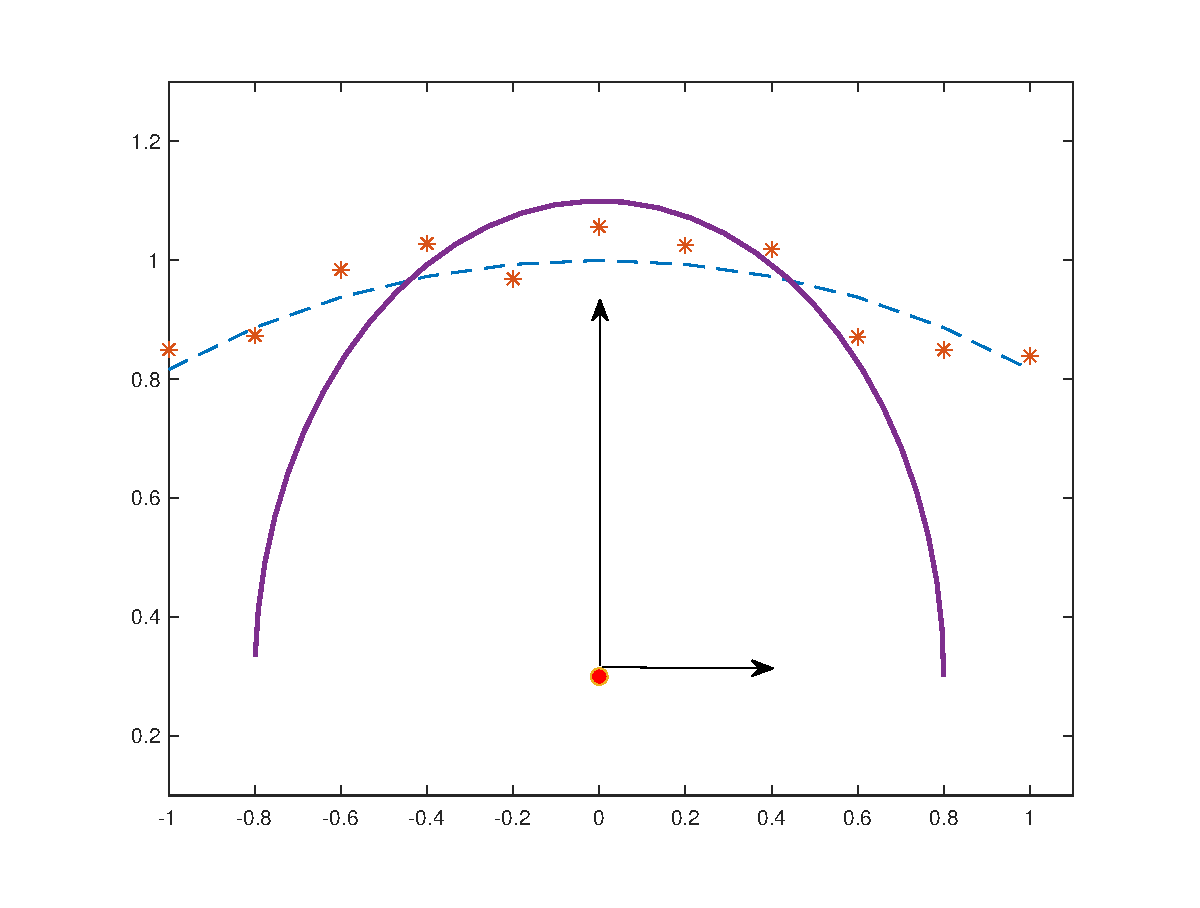
\includegraphics[width=0.32\linewidth]{../figures/demo1.eps} 
\hspace{-4mm}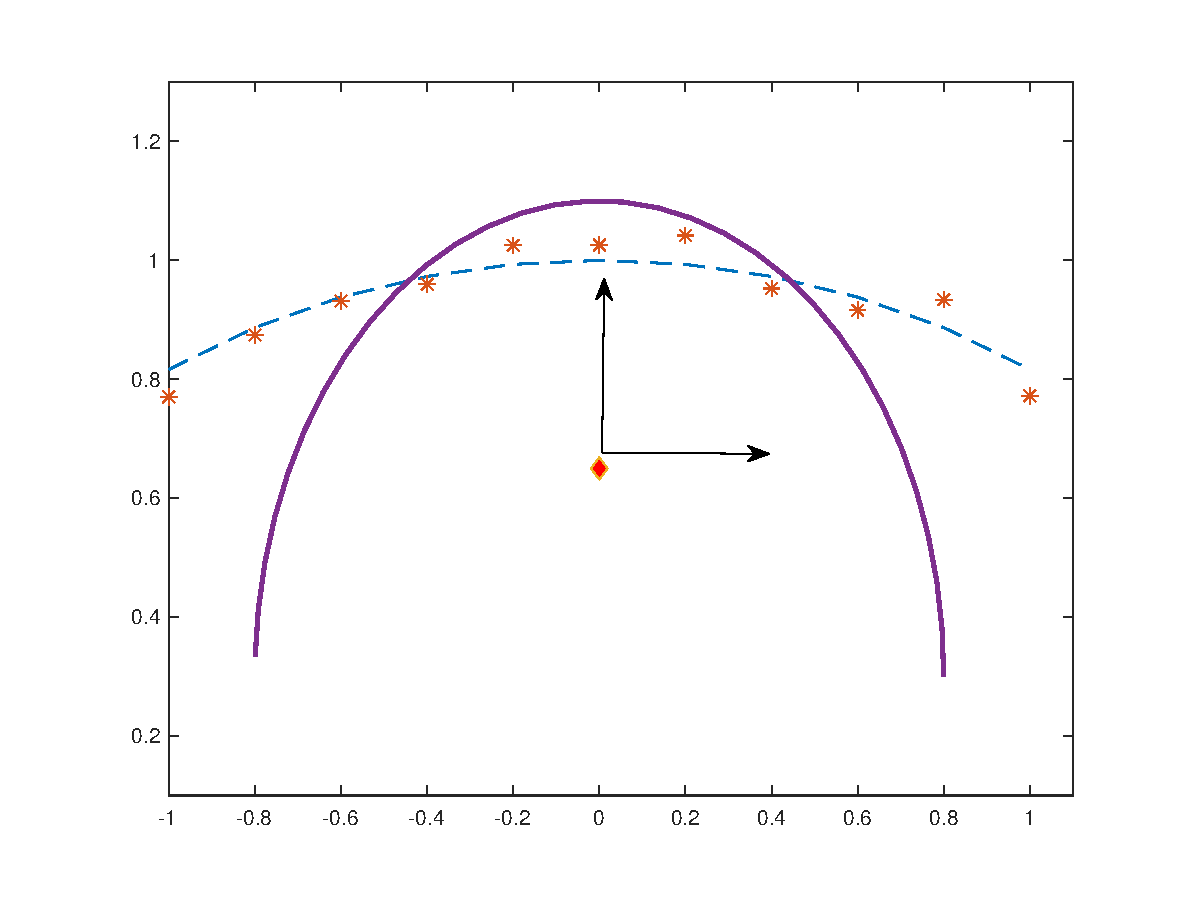
\includegraphics[width=0.32\linewidth]{../figures/demo2.eps} 
\hspace{-4mm}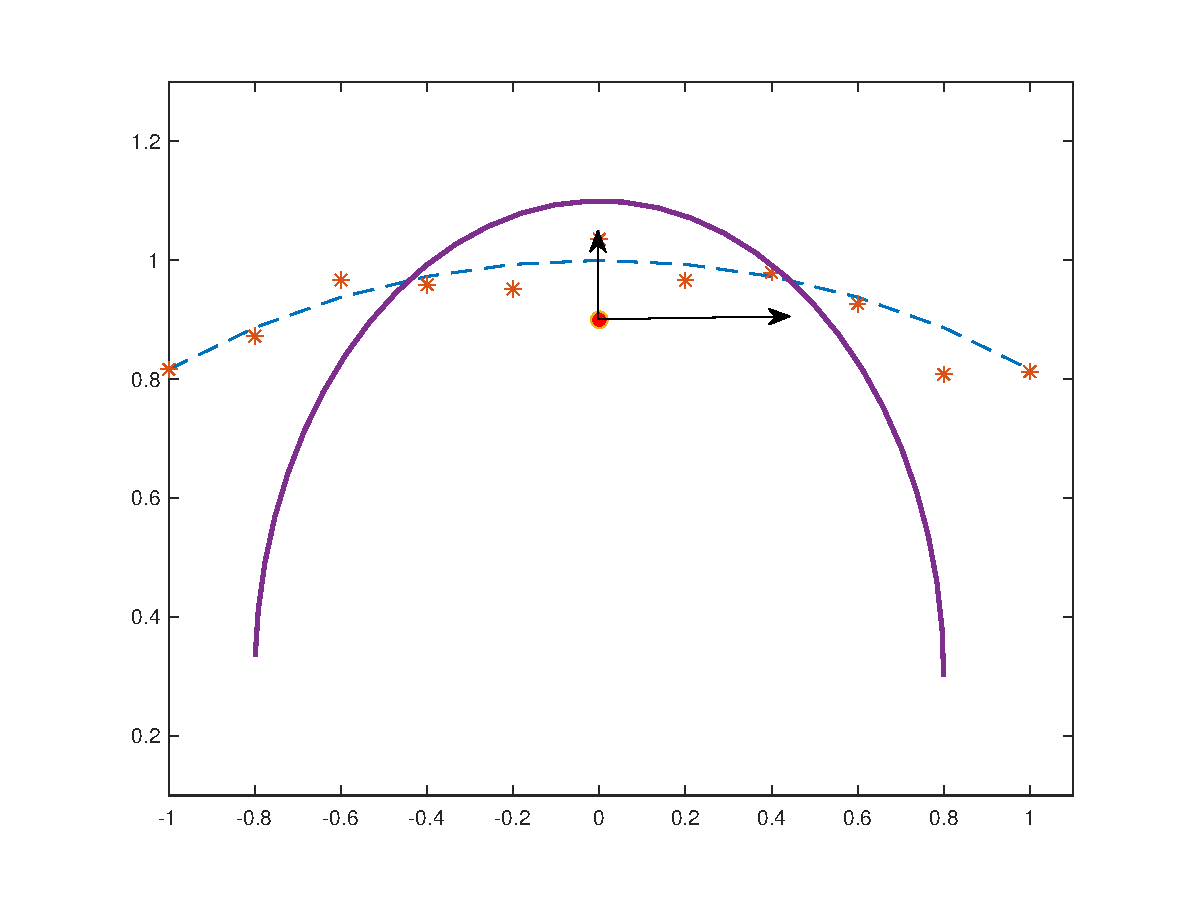
\includegraphics[width=0.32\linewidth]{../figures/demo3.eps} 
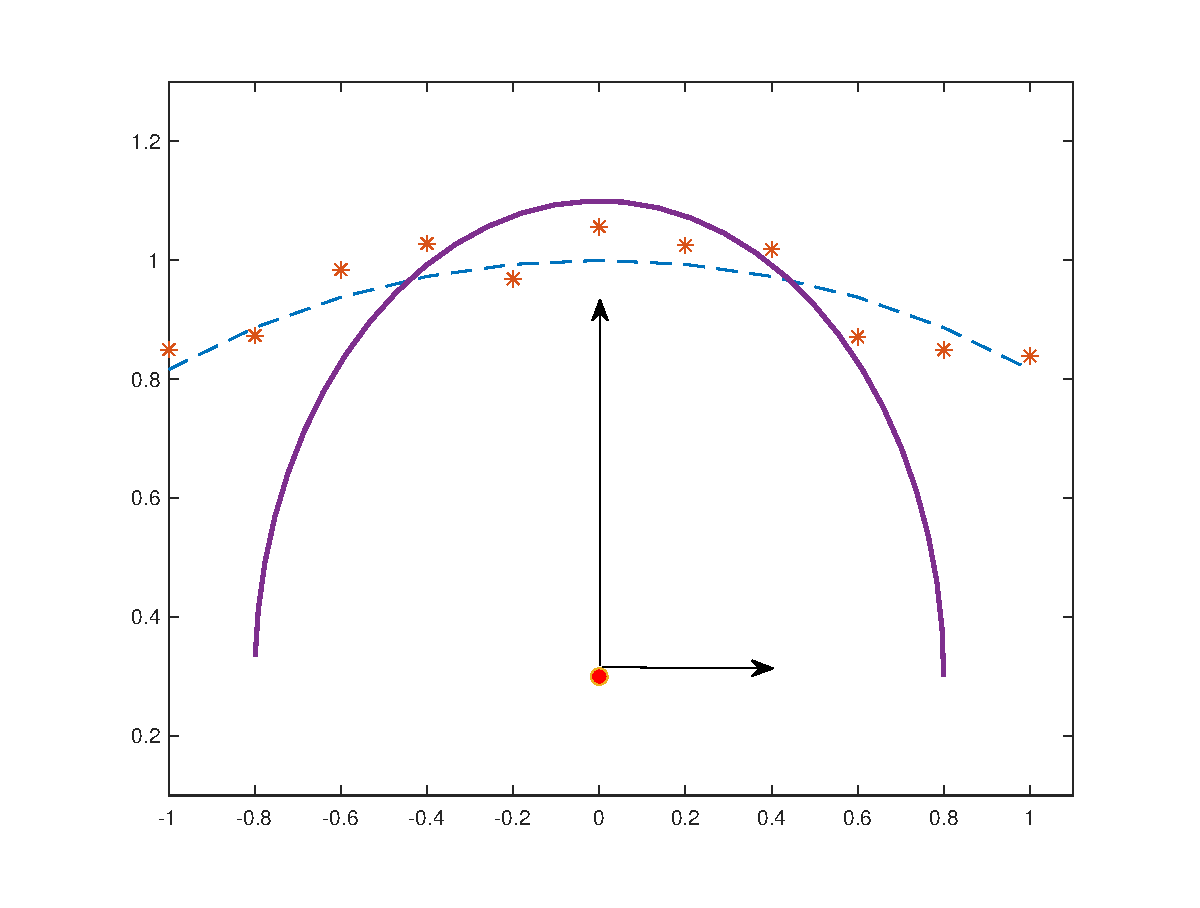
\includegraphics{../figures/demo1.eps}
%\setcaptionwidth{6in}
\caption{The process of $J(x)$'s eigenspace's variation with $x$ approaching the manifold }
\label{Shifting Eigenvectors}
\end{figure}

\begin{figure}
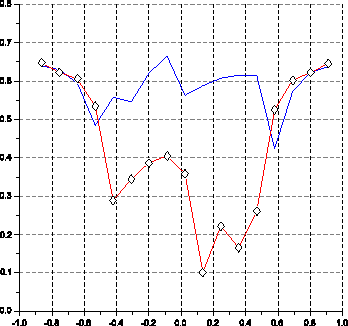
\includegraphics{figure1}
\caption{Pathway of the penicillin G biosynthesis.}
\label{penG}
\end{figure}

Sample of cross-reference to figure.
Figure~\ref{penG} shows that it is not easy to get something on paper.

\section{Equations and the like}

Two equations:
\begin{equation}
    C_{s}  =  K_{M} \frac{\mu/\mu_{x}}{1-\mu/\mu_{x}} \label{ccs}
\end{equation}
and
\begin{equation}
    G = \frac{P_{\mathrm{opt}} - P_{\mathrm{ref}}}{P_{\mathrm{ref}}}  100(\%).
\end{equation}

Equation arrays:
\begin{eqnarray}
  \frac{dS}{dt} & = & - \sigma X + s_{F} F,\\
  \frac{dX}{dt} & = &   \mu    X,\\
  \frac{dP}{dt} & = &   \pi    X - k_{h} P,\\
  \frac{dV}{dt} & = &   F.
\end{eqnarray}
One long equation:
\begin{eqnarray}
 \mu_{\text{normal}} & = & \mu_{x} \frac{C_{s}}{K_{x}C_{x}+C_{s}}  \nonumber\\
                     & = & \mu_{\text{normal}} - Y_{x/s}\bigl(1-H(C_{s})\bigr)(m_{s}+\pi /Y_{p/s})\\
                     & = & \mu_{\text{normal}}/Y_{x/s}+ H(C_{s}) (m_{s}+ \pi /Y_{p/s}).\nonumber
\end{eqnarray}
%%%%%%%%%%%%%%%%%%%%%%%%%%%%%%%%%%%%%%%%%%%%%%
%% Example with single Appendix:            %%
%%%%%%%%%%%%%%%%%%%%%%%%%%%%%%%%%%%%%%%%%%%%%%
\begin{appendix}
\section*{Title}\label{appn} %% if no title is needed, leave empty \section*{}.
Appendices should be provided in \verb|{appendix}| environment,
before Acknowledgements.

If there is only one appendix,
then please refer to it in text as \ldots\ in the \hyperref[appn]{Appendix}.
\end{appendix}
%%%%%%%%%%%%%%%%%%%%%%%%%%%%%%%%%%%%%%%%%%%%%%
%% Example with multiple Appendixes:        %%
%%%%%%%%%%%%%%%%%%%%%%%%%%%%%%%%%%%%%%%%%%%%%%
\begin{appendix}
\section{Title of the first appendix}\label{appA}
If there are more than one appendix, then please refer to it
as \ldots\ in Appendix \ref{appA}, Appendix \ref{appB}, etc.

\section{Title of the second appendix}\label{appB}
\subsection{First subsection of Appendix \protect\ref{appB}}

Use the standard \LaTeX\ commands for headings in \verb|{appendix}|.
Headings and other objects will be numbered automatically.
\begin{equation}
\mathcal{P}=(j_{k,1},j_{k,2},\dots,j_{k,m(k)}). \label{path}
\end{equation}

Sample of cross-reference to the formula (\ref{path}) in Appendix \ref{appB}.
\end{appendix}

%%%%%%%%%%%%%%%%%%%%%%%%%%%%%%%%%%%%%%%%%%%%%%
%% Support information (funding), if any,   %%
%% should be provided in the                %%
%% Acknowledgements section.                %%
%%%%%%%%%%%%%%%%%%%%%%%%%%%%%%%%%%%%%%%%%%%%%%
\section*{Acknowledgements}
The authors would like to thank the anonymous referees, an Associate
Editor and the Editor for their constructive comments that improved the
quality of this paper.

The first author was supported by NSF Grant DMS-??-??????.

The second author was supported in part by NIH Grant ???????????.


%%%%%%%%%%%%%%%%%%%%%%%%%%%%%%%%%%%%%%%%%%%%%%
%% Supplementary Material, if any, should   %%
%% be provided in {supplement} environment  %%
%% with title and short description.        %%
%%%%%%%%%%%%%%%%%%%%%%%%%%%%%%%%%%%%%%%%%%%%%%
\begin{supplement}
\textbf{Title of Supplement A}.
Short description of Supplement A.
\end{supplement}
\begin{supplement}
\textbf{Title of Supplement B}.
Short description of Supplement B.
\end{supplement}

%%%%%%%%%%%%%%%%%%%%%%%%%%%%%%%%%%%%%%%%%%%%%%%%%%%%%%%%%%%%%
%%                  The Bibliography                       %%
%%                                                         %%
%%  imsart-???.bst  will be used to                        %%
%%  create a .BBL file for submission.                     %%
%%                                                         %%
%%  Note that the displayed Bibliography will not          %%
%%  necessarily be rendered by Latex exactly as specified  %%
%%  in the online Instructions for Authors.                %%
%%                                                         %%
%%  MR numbers will be added by VTeX.                      %%
%%                                                         %%
%%  Use \cite{...} to cite references in text.             %%
%%                                                         %%
%%%%%%%%%%%%%%%%%%%%%%%%%%%%%%%%%%%%%%%%%%%%%%%%%%%%%%%%%%%%%

%% if your bibliography is in bibtex format, uncomment commands:
%\bibliographystyle{imsart-number} % Style BST file (imsart-number.bst or imsart-nameyear.bst)
%\bibliography{bibliography}       % Bibliography file (usually '*.bib')

%% or include bibliography directly:
\begin{thebibliography}{4}
%%
\bibitem{r1}
\textsc{Billingsley, P.} (1999). \textit{Convergence of
Probability Measures}, 2nd ed.
Wiley, New York.

\bibitem{r2}
\textsc{Bourbaki, N.}  (1966). \textit{General Topology}  \textbf{1}.
Addison--Wesley, Reading, MA.

\bibitem{r3}
\textsc{Ethier, S. N.} and \textsc{Kurtz, T. G.} (1985).
\textit{Markov Processes: Characterization and Convergence}.
Wiley, New York.

\bibitem{r4}
\textsc{Prokhorov, Yu.} (1956).
Convergence of random processes and limit theorems in probability
theory. \textit{Theory  Probab.  Appl.}
\textbf{1} 157--214.
\end{thebibliography}

\end{document}

